\documentclass[10pt]{report}
\usepackage[nottoc,numbib]{tocbibind}
\usepackage{graphicx}
\usepackage{natbib}
\usepackage{graphics}
\usepackage{url}
\usepackage{hyperref}
\usepackage{amsmath}
\usepackage{mathtools}
\usepackage[brazil]{babel} 
\usepackage{float}
\usepackage[scale=2]{ccicons}
\usepackage[utf8]{inputenc}
\usepackage[T1]{fontenc}
\usepackage[a4paper, width=200mm,top=5mm,bottom=5mm]{geometry}
%\usepackage{biblatex} COOOOOORNOOOOOOOO
\usepackage{titlesec}
\usepackage{minted}
\usepackage{listings}
\usepackage{xcolor}
\usepackage{caption}

\definecolor{codegreen}{rgb}{0,0.6,0}
\definecolor{codegray}{rgb}{0.5,0.5,0.5}
\definecolor{codepurple}{rgb}{0.58,0,0.82}
\definecolor{backcolour}{rgb}{0.95,0.95,0.92}

\lstdefinestyle{mystyle}{
    backgroundcolor=\color{backcolour},   
    commentstyle=\color{codegreen},
    keywordstyle=\color{magenta},
    numberstyle=\tiny\color{codegray},
    stringstyle=\color{codepurple},
    basicstyle=\ttfamily\scriptsize,
    breakatwhitespace=false,         
    breaklines=true,                 
    captionpos=b,                    
    keepspaces=true,                 
    numbers=left,                    
    numbersep=5pt,                  
    showspaces=false,                
    showstringspaces=false,
    showtabs=false,                  
    tabsize=2,
    extendedchars=true,
    inputencoding=latin1
}

\graphicspath{{pratica3/prints}{pratica4/prints}{pratica5/prints}}

\lstset{style=mystyle}
\lstset{literate=
  {á}{{\'a}}1 {é}{{\'e}}1 {í}{{\'i}}1 {ó}{{\'o}}1 {ú}{{\'u}}1
  {Á}{{\'A}}1 {É}{{\'E}}1 {Í}{{\'I}}1 {Ó}{{\'O}}1 {Ú}{{\'U}}1
  {à}{{\`a}}1 {è}{{\`e}}1 {ì}{{\`i}}1 {ò}{{\`o}}1 {ù}{{\`u}}1
  {À}{{\`A}}1 {È}{{\'E}}1 {Ì}{{\`I}}1 {Ò}{{\`O}}1 {Ù}{{\`U}}1
  {ä}{{\"a}}1 {ë}{{\"e}}1 {ï}{{\"i}}1 {ö}{{\"o}}1 {ü}{{\"u}}1
  {Ä}{{\"A}}1 {Ë}{{\"E}}1 {Ï}{{\"I}}1 {Ö}{{\"O}}1 {Ü}{{\"U}}1
  {â}{{\^a}}1 {ê}{{\^e}}1 {î}{{\^i}}1 {ô}{{\^o}}1 {û}{{\^u}}1
  {Â}{{\^A}}1 {Ê}{{\^E}}1 {Î}{{\^I}}1 {Ô}{{\^O}}1 {Û}{{\^U}}1
  {Ã}{{\~A}}1 {ã}{{\~a}}1 {Õ}{{\~O}}1 {õ}{{\~o}}1
  {œ}{{\oe}}1 {Œ}{{\OE}}1 {æ}{{\ae}}1 {Æ}{{\AE}}1 {ß}{{\ss}}1
  {ű}{{\H{u}}}1 {Ű}{{\H{U}}}1 {ő}{{\H{o}}}1 {Ő}{{\H{O}}}1
  {ç}{{\c c}}1 {Ç}{{\c C}}1 {ø}{{\o}}1 {å}{{\r a}}1 {Å}{{\r A}}1
  {€}{{\euro}}1 {£}{{\pounds}}1 {«}{{\guillemotleft}}1
  {»}{{\guillemotright}}1 {ñ}{{\~n}}1 {Ñ}{{\~N}}1 {¿}{{?`}}1
}

\title{Sistemas Distribuídos - Relatório 2}

\author{Claudio Quessada Cabello \textbf{RA:} 11000516 &
        Claudio Quessada Cabello \textbf{RA:} 11000516 &
        Claudio Quessada Cabello \textbf{RA:} 11000516 }

\begin{document} 

\maketitle

\tableofcontents
\listoffigures

\chapter*{Aula prática 2 - SÓ DE EXEMPLO!!!}
\addcontentsline{toc}{chapter}{Aula prática 2 Remover!}
\subsection*{1. Executar os diferentes servidores em uma máquina diferente da
máquina cliente.}
\addcontentsline{toc}{section}{1. Executar os servidores}

Os \textit{}{Batch Scripts} foram reescritos como \textit{Shell Scripts} com o intuito de serem executados tanto no Linux nativo (Manjaro Linux) quanto no \textit{Windows Subsystem for Linux} (WSL). Os scripts todos estão disponíveis no arquivo zipado, junto com os Batch Scripts


\subsubsection{1.1 - Servidor: executar o rmi.bat e depois o server.bat.}
\addcontentsline{toc}{subsection}{1.1 Execução do servidor}

Primeiramente foi executado o comando \textit{rmiregistry}, seguido pelo script \texttt{server.sh} para iniciar comunicação com o registro e o armazenamento das informações do servidor.

\vspace{2em}
\begin{minipage}{\textwidth}
    \hspace{-1em}
    \centering
    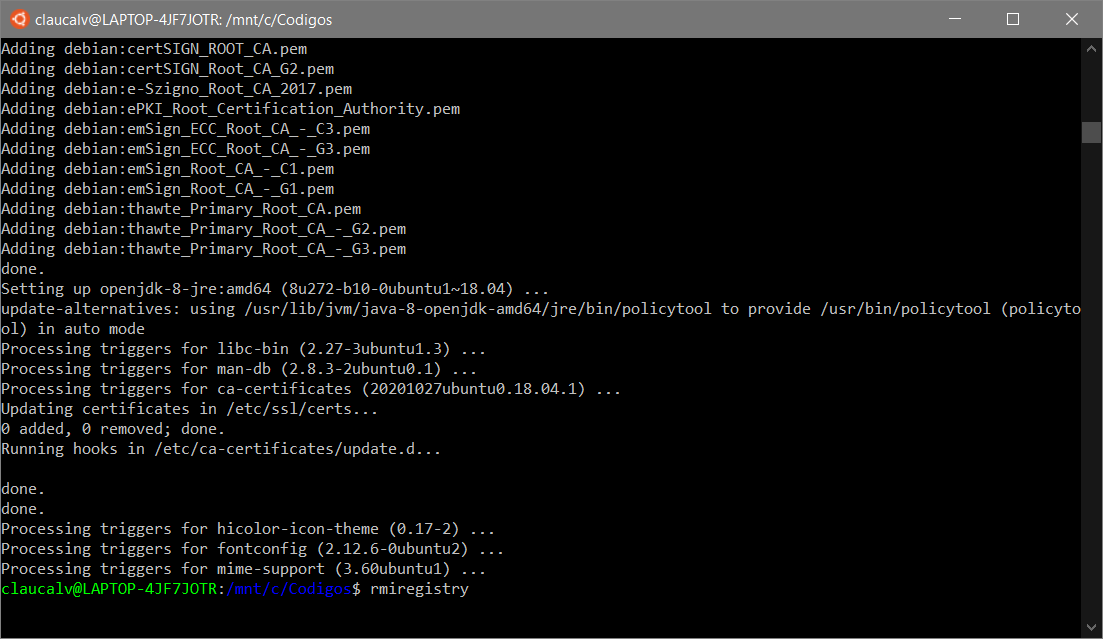
\includegraphics[scale=.35]{prints/rmiregistry.PNG}
    \hspace{1em}
    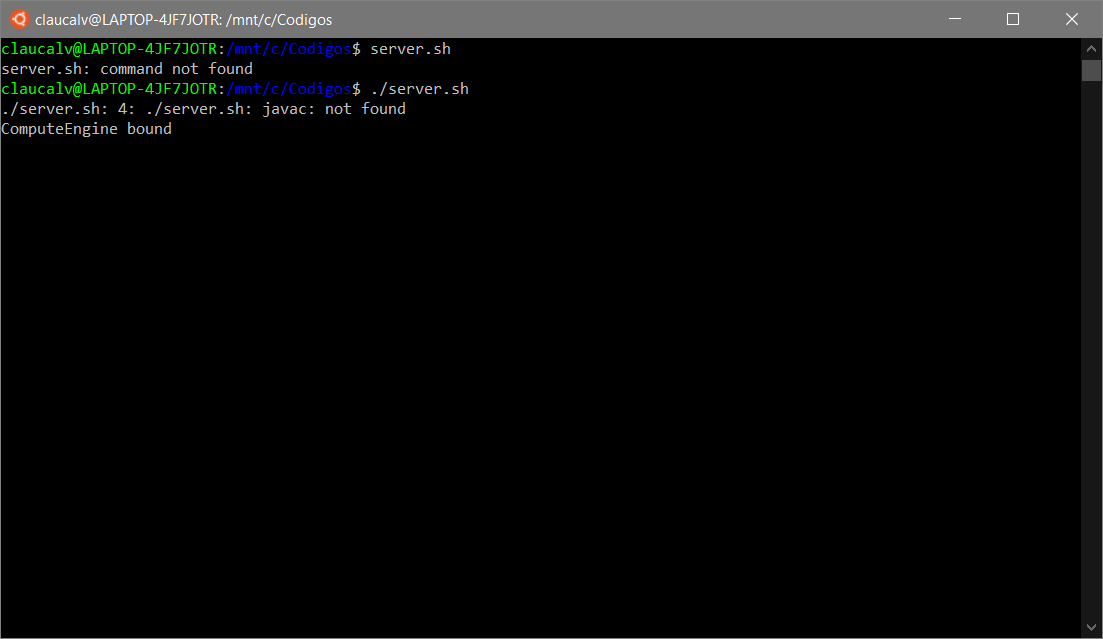
\includegraphics[scale=.35]{prints/server.PNG}
    \captionof{figure}{Execução do rmiregistry e do server}
    \label{threadspng}
    \hspace{1em}
\end{minipage}
\vspace{0.5em}


\subsubsection{1.2 - Cliente: executar o client.bat. Discorra sobre os tempos obtidos na
execução de forma remota e local.}
\addcontentsline{toc}{subsection}{1.2 Execução do client}

Foi feita a execução do arquivo \textit{client.sh} adaptado do \textit{client.bat} para execução no WSL.

\vspace{2em}
\begin{minipage}{\textwidth}
    \hspace{-1em}
    \centering
    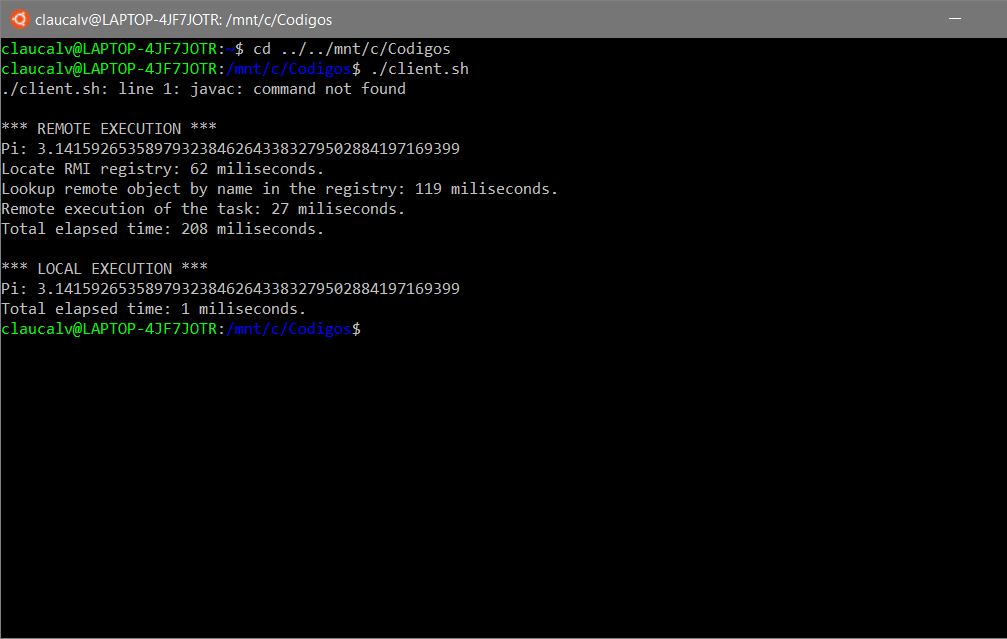
\includegraphics[trim= 0 150 250 0, clip, scale=.4]{prints/client.PNG}
    \captionof{figure}{Execução do cliente}
    \label{threadspng}
    \hspace{1em}
\end{minipage}
\vspace{0.5em}


\subsection*{2. Executar a classe \textit{serialization.SerialObject} com os parâmetros adequados (nome de arquivo e operação).}
\addcontentsline{toc}{section}{2. Execução da serialização}



\vspace{2em}
\begin{minipage}{\textwidth}
    \hspace{-1em}
    \centering
    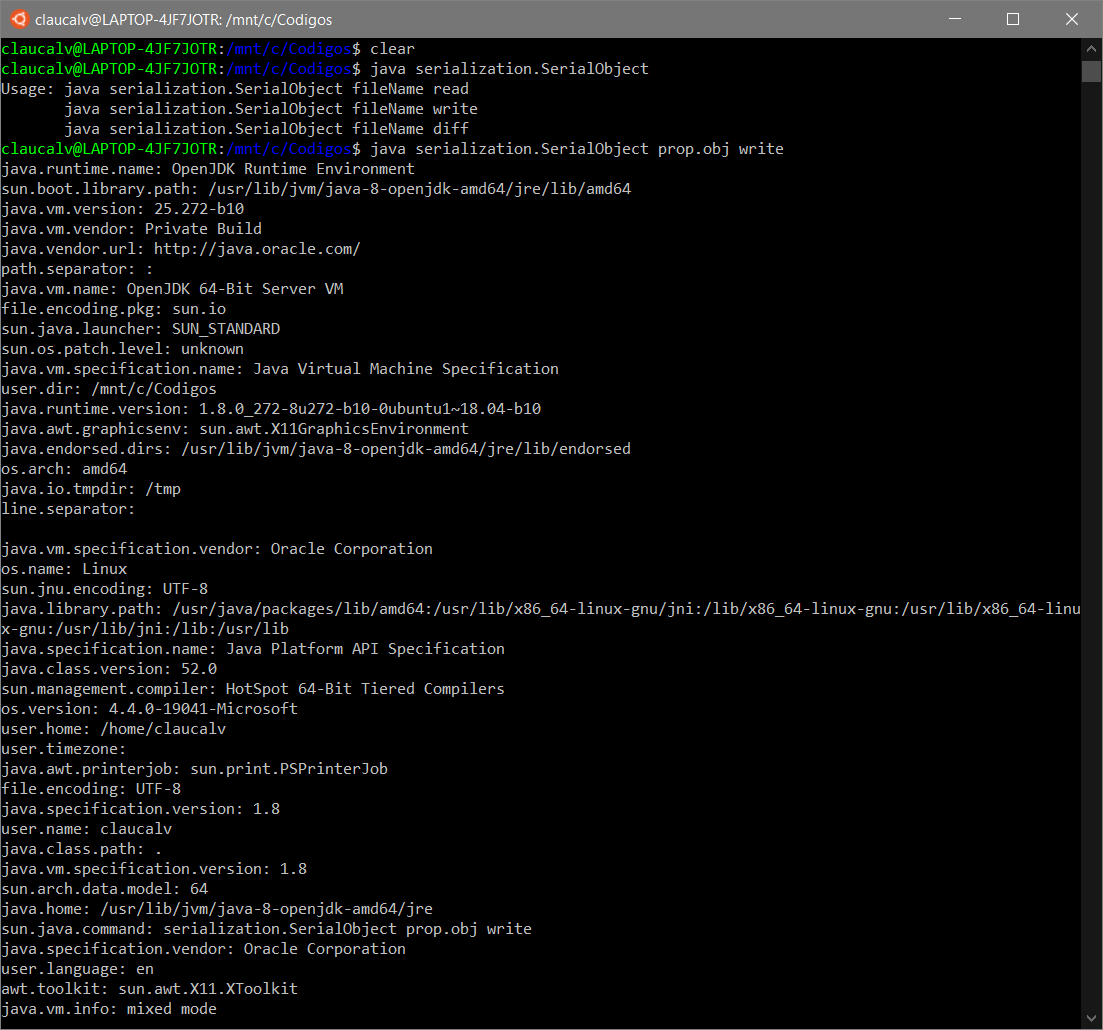
\includegraphics[scale=.35]{prints/serial1.PNG}
    \hspace{1em}
    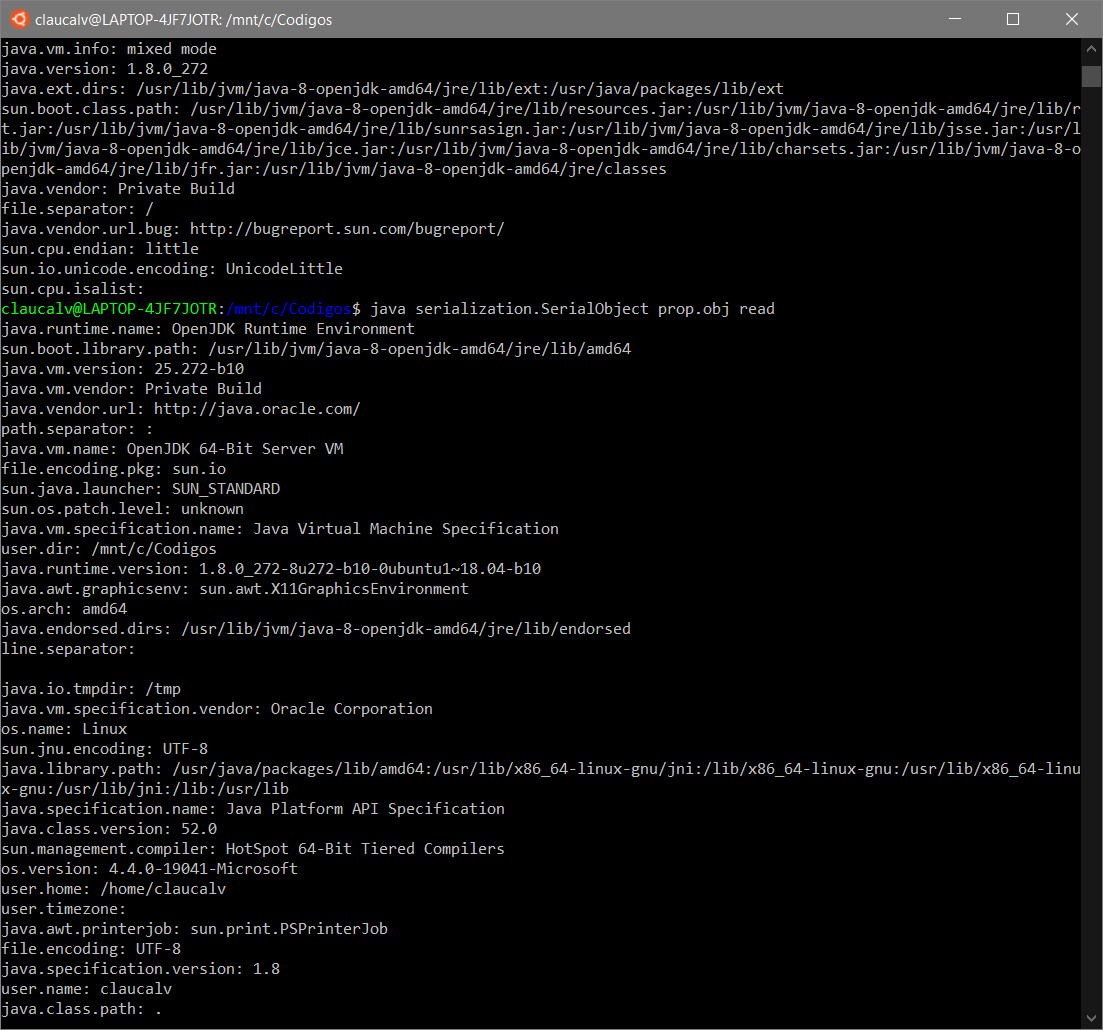
\includegraphics[scale=.35]{prints/serial2.PNG}
    \hspace{1em}
    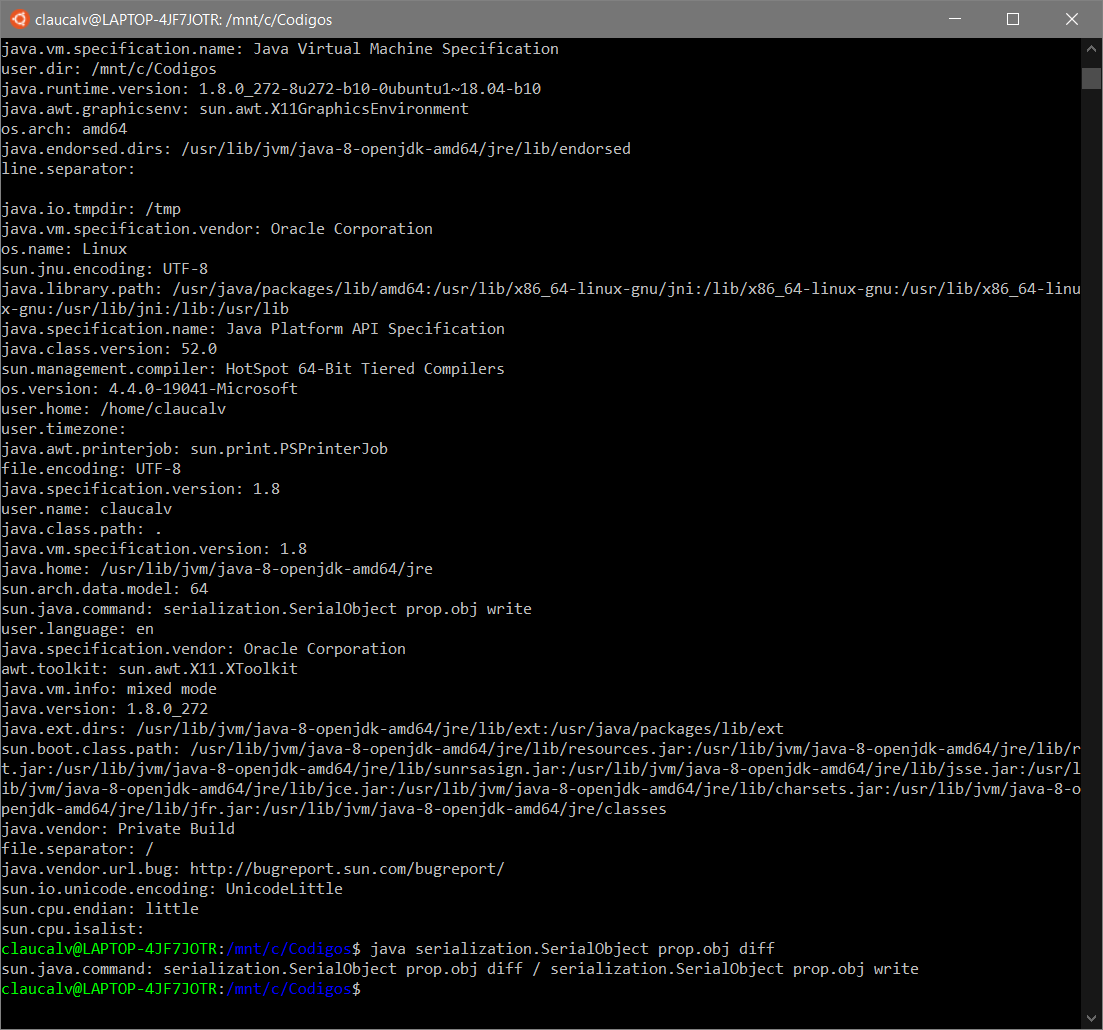
\includegraphics[scale=.35]{prints/serial3.PNG}
    \captionof{figure}{Execução do SerialObject}
    \label{threadspng}
    \hspace{1em}
\end{minipage}
\vspace{0.5em}

\subsubsection{2.1 - Qual o papel de cada operação (write, read e diff)?}
\addcontentsline{toc}{subsection}{2.1 Diferenças de operação}

A operação \textit{write} grava em arquivo o objeto \textit{System.properties}. A operação \textit{read} recupera o arquivo \textit{properties} (uma \textit{hashtable}) e imprime na tela. A operação \textit{diff} faz a diferença entre o arquivo e o \textit{System.properties} atual.

\subsection*{3. Implementar um sistema cliente-servidor em que o cliente envia seu objeto \textit{Properties} a um servidor por meio de \textit{socket}. O servidor compara o objeto enviado com seu próprio \textit{Properties} e devolve o resultado da operação \textit{diff} ao cliente, que é impresso na tela}
\addcontentsline{toc}{section}{3. Implementação cliente-servidor}

\vspace{-0.5em}
\begin{minipage}{\textwidth}
  \hspace{-1em}
  \centering
  \lstinputlisting[language=Java]{codigos/serialization/SerialObjectServer.java}
  \captionof{figure}{Implementação do servidor da serialização}
  \label{prog1}
  \hspace{1em}
\end{minipage}
\vspace{0.5em}

\vspace{-0.5em}
\begin{minipage}{\textwidth}
  \hspace{-1em}
  \centering
  \lstinputlisting[language=Java]{codigos/serialization/SerialObjectClient.java}
  \captionof{figure}{Implementação do cliente da serialização}
  \label{prog1}
  \hspace{1em}
\end{minipage}
\vspace{0.5em}

\vspace{2em}
\begin{minipage}{\textwidth}
    \hspace{-1em}
    \centering
    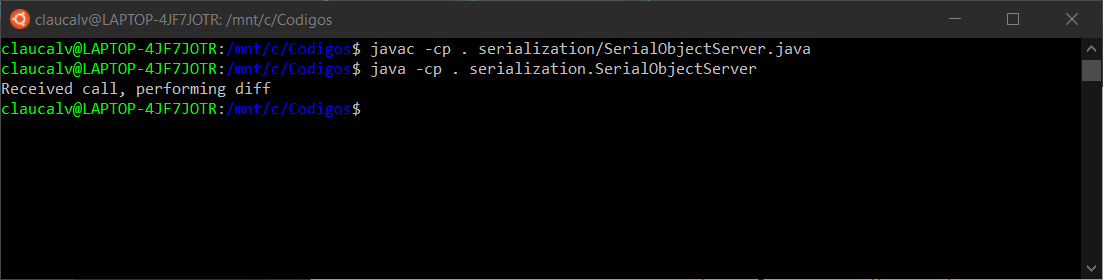
\includegraphics[scale=.35]{prints/serial_server.PNG}
    \hspace{1em}
    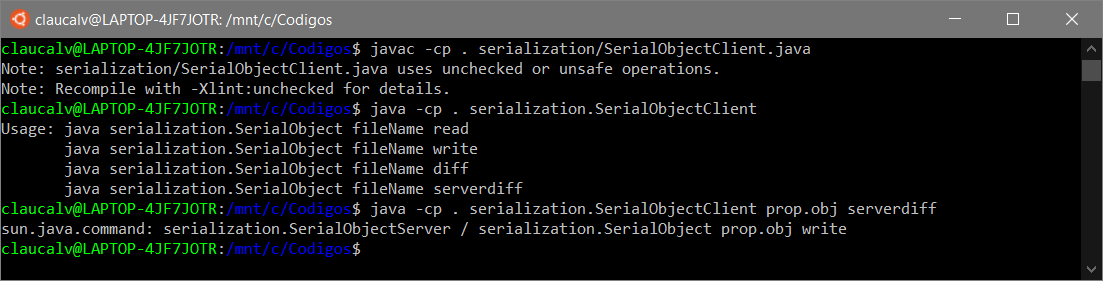
\includegraphics[scale=.35]{prints/serial_client.PNG}
    \captionof{figure}{Execução do servidor e cliente da serialização}
    \label{threadspng}
    \hspace{1em}
\end{minipage}
\vspace{0.5em}

\chapter*{Aula prática 3}
\addcontentsline{toc}{chapter}{Aula prática 3}
\subsection*{1. Ephemeral versus Persistent (Regular) znodes}
\addcontentsline{toc}{section}{1. Ephemeral versus Persistent (Regular) znodes}

\subsubsection{1.1 - Inicialize a interface de comando de linha (CLI): bin/zkCli.sh
-server 127.0.0.1:2181}
\addcontentsline{toc}{subsection}{1.1 Inicialize o CLI}

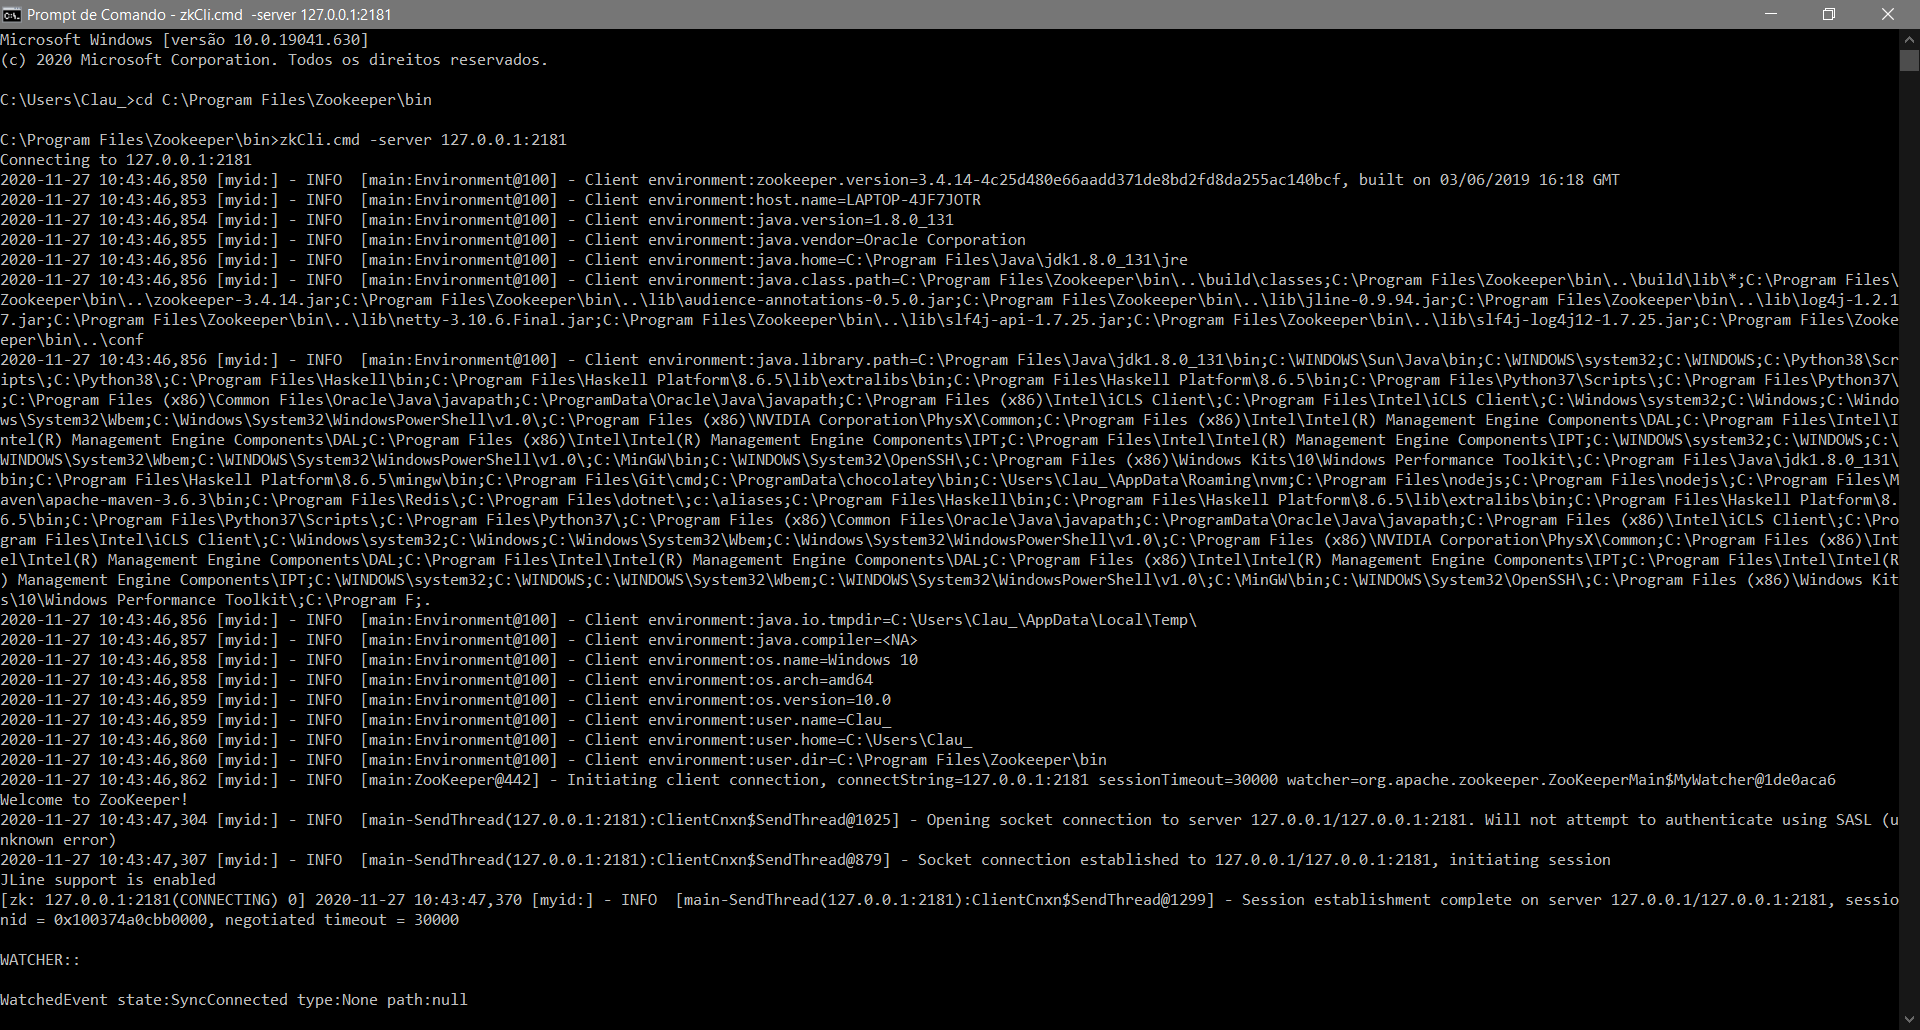
\includegraphics[width=20cm]{pratica3/prints/client1_started.PNG}

\subsubsection{1.2 - Crie um znode persistente para este exercício: create /mcta025 data}
\addcontentsline{toc}{subsection}{1.2 Crie um znode persistente para este exercício}

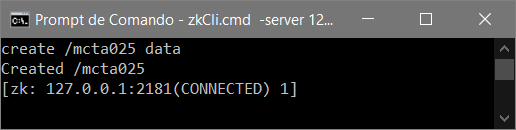
\includegraphics{pratica3/prints/roteiro 1.2.PNG}

\subsubsection{1.3 - Crie um outro znode persistente: create /mcta025/ex1 data}
\addcontentsline{toc}{subsection}{1.3 Crie um outro znode persistente}

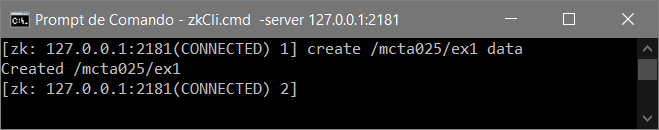
\includegraphics{pratica3/prints/roteiro 1.3.PNG}

\subsubsection{1.4 - Crie um znode efêmero: create -e /mcta025/ex1/ephemeral data}
\addcontentsline{toc}{subsection}{1.4 Crie um znode efêmero}

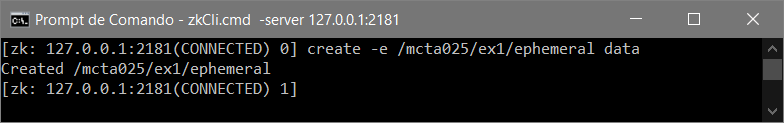
\includegraphics{pratica3/prints/roteiro 1.4.PNG}

\subsubsection{1.5 - Liste os filhos do seu sistema de arquivo (na API, getChildren): ls
<path>}
\addcontentsline{toc}{subsection}{1.5 Liste os filhos do seu sistema de arquivo}

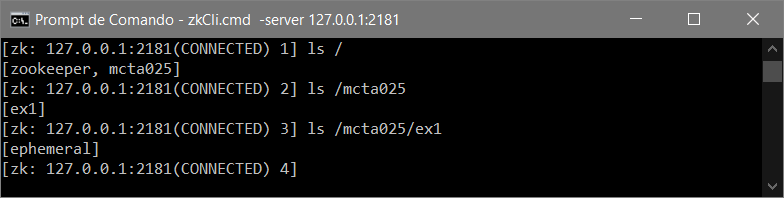
\includegraphics{pratica3/prints/roteiro 1.5.PNG}

\subsubsection{1.6 - Saia do cliente usando o comando quit}
\addcontentsline{toc}{subsection}{1.6 Saia do cliente usando o comando quit}

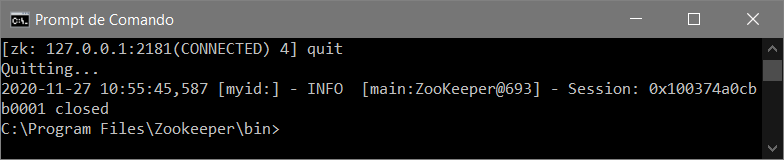
\includegraphics{pratica3/prints/roteiro 1.6.PNG}

\subsubsection{1.7 - Reinicie a CLI e liste novamente os filhos do sistema de arquivo. O que aconteceu?}
\addcontentsline{toc}{subsection}{1.7 Reinicie a CLI e liste novamente os filhos do sistema de arquivo}
Ao reiniciar a CLI, os filhos do sistema de arquivos é zerada.
\newline

\begin{center}
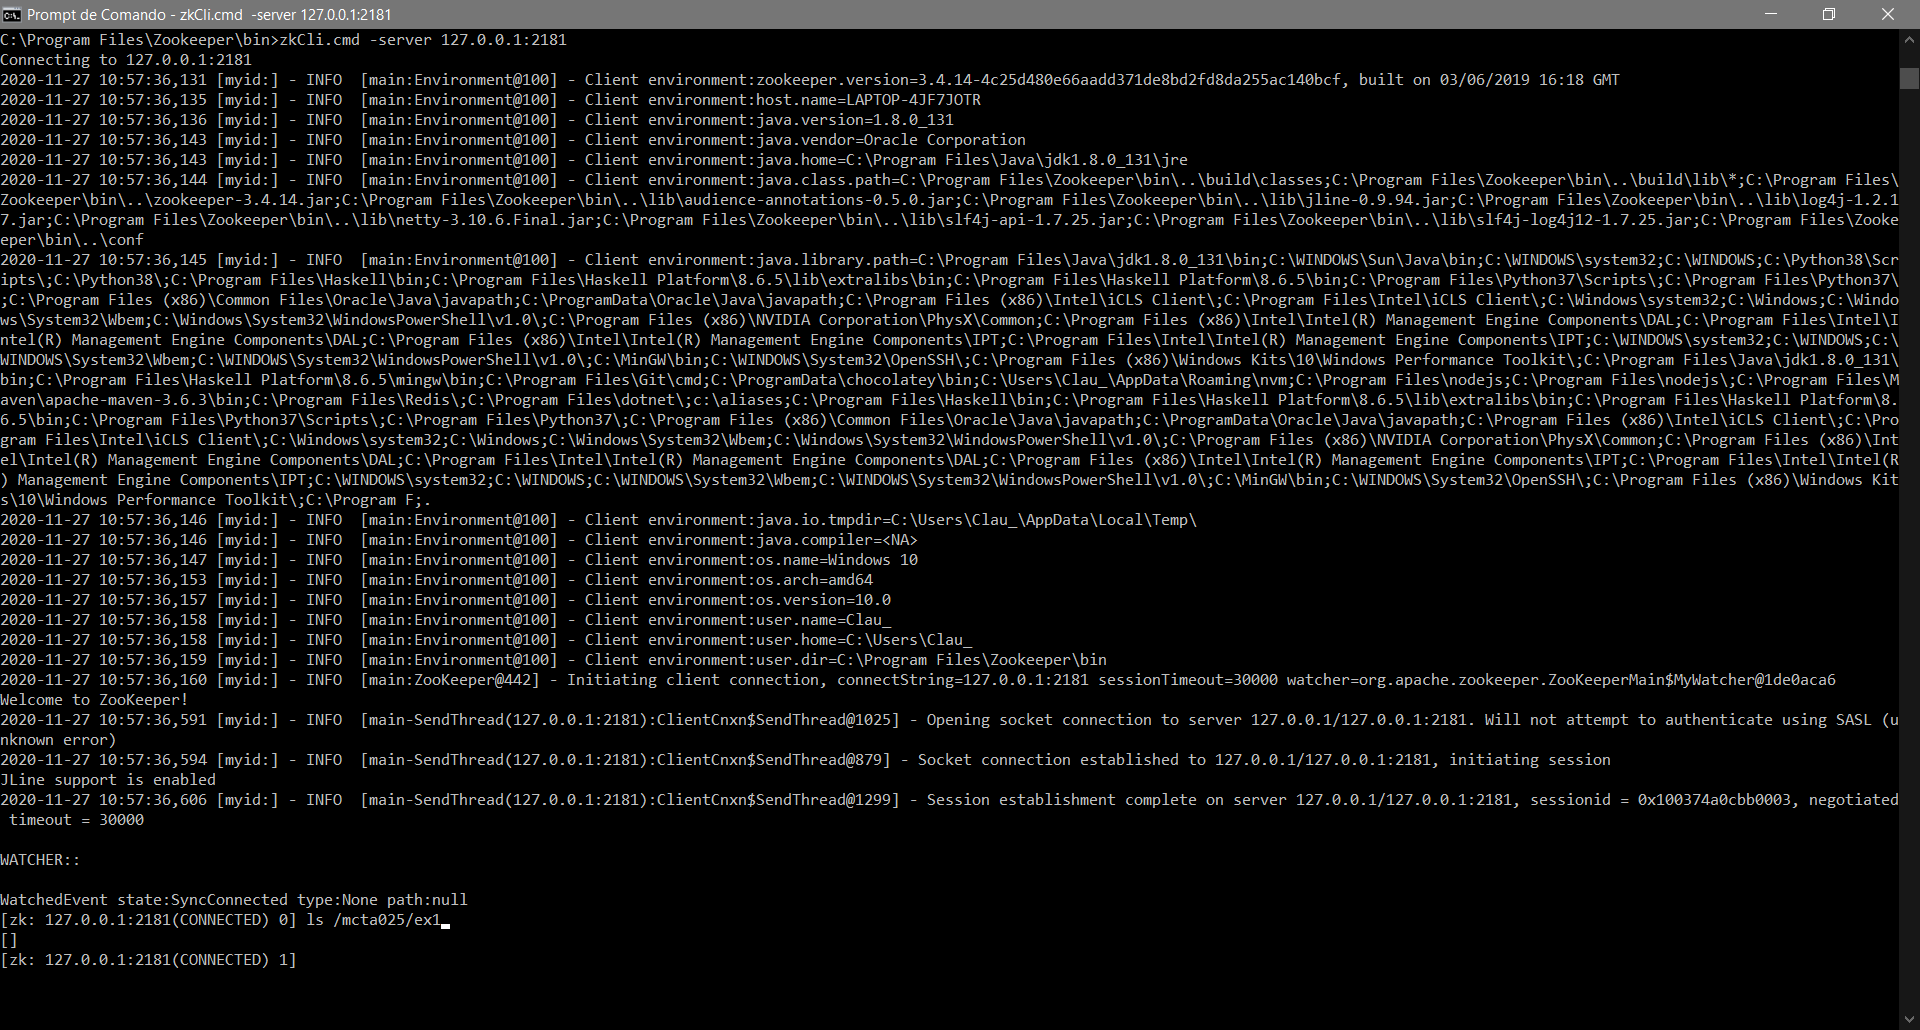
\includegraphics[width=20cm]{pratica3/prints/roteiro 1.7.PNG}
\end{center}

\subsubsection{1.8 - Crie um novo znode efêmero: create -e /mcta025/ex1/ephemeral1 data. Então, crie um filho para o znode que acabou de ser criado: create /mcta025/ex1/ephemeral1/child data. O que aconteceu?}
\addcontentsline{toc}{subsection}{1.8  Tente criar um filho de um znode efêmero}

Znodes efêmeros não podem ter znodes filhos.
\newline
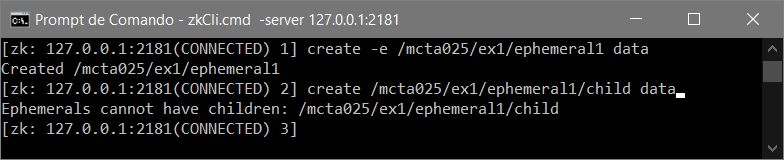
\includegraphics{pratica3/prints/roteiro 1.8.PNG}

\subsection*{2. Sequential suffix}
\addcontentsline{toc}{section}{2. Sequential suffix}

\subsubsection{2.1 - Crie um outro znode persistente: create /mcta025/ex2 data}
\addcontentsline{toc}{subsection}{2.1  Crie um outro znode persistente}

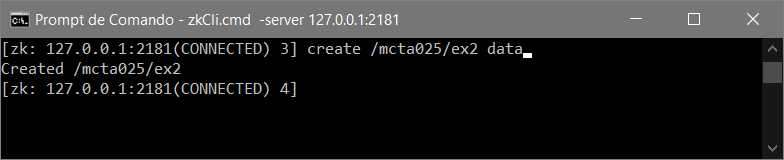
\includegraphics{pratica3/prints/roteiro 2.1.PNG}

\subsubsection{2.2 - Crie znodes sequenciais (com sufixo sequencial): create -s
/mcta025/ex2/child data. Repita o comando várias vezes. Qual o
comprimento do sufixo?}
\addcontentsline{toc}{subsection}{2.2  Crie znodes sequenciais}
O comprimento do sufixo é de 10 caracteres.
\newline
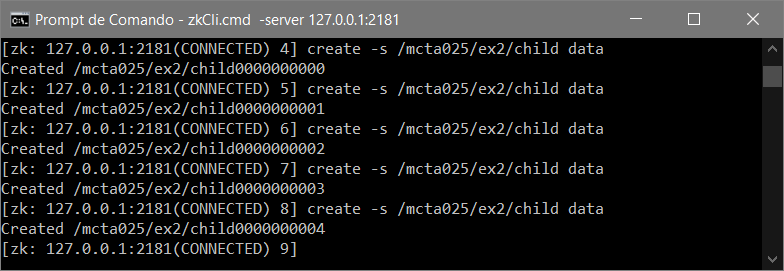
\includegraphics{pratica3/prints/roteiro 2.2.PNG}

\subsubsection{2.3 - Crie znodes sequenciais efêmeros: create -s -e
/mcta025/ex2/child data. Repita o comando várias vezes}
\addcontentsline{toc}{subsection}{2.3 Crie znodes sequenciais efêmeros}

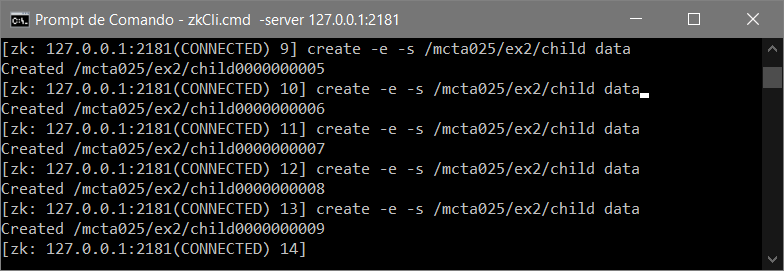
\includegraphics{pratica3/prints/roteiro 2.3.PNG}

\subsubsection{2.4 - Remova alguns znodes com o comando: delete <path>.}
\addcontentsline{toc}{subsection}{2.4   Remova alguns znodes}

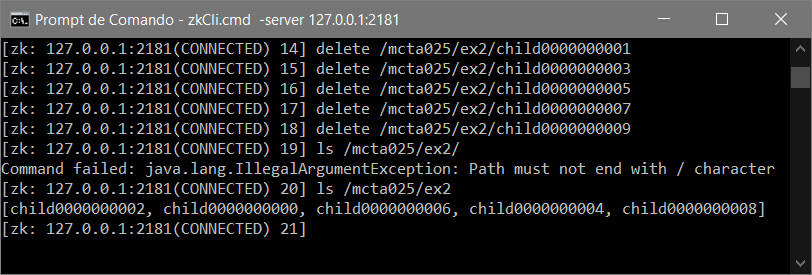
\includegraphics{pratica3/prints/roteiro 2.4.PNG}

\subsubsection{2.5 - Crie mais alguns znodes sequenciais. Como fica a numeração deles?}
\addcontentsline{toc}{subsection}{2.5  Crie mais alguns znodes sequenciais}
A numeração permanece incremental, independente dos znodes que foram deletados.
\newline
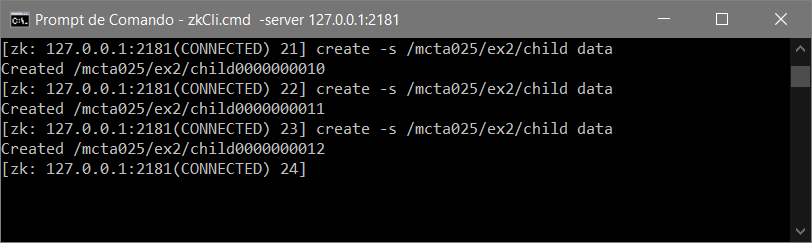
\includegraphics{pratica3/prints/roteiro 2.5.PNG}

\subsubsection{2.6 - Crie znodes sequenciais com outro prefixo: create -s
/mcta025/ex2/son data. Como fica a numeração deles?}
\addcontentsline{toc}{subsection}{2.6  Crie znodes sequenciais com outro prefixo}
A numeração permanece incremental, independente do prefixo.
\newline
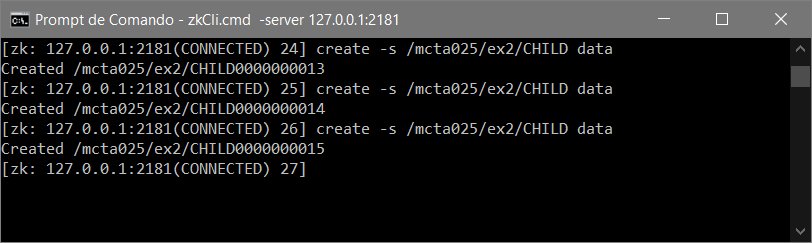
\includegraphics{pratica3/prints/roteiro 2.6.PNG}

\subsubsection{2.7 - Crie outros znodes sequenciais em /mcta025. A numeração (isto é, o escopo) está relacionada com a numeração anterior?}
\addcontentsline{toc}{subsection}{2.7 Crie outros znodes sequenciais e correlacione com a numeração anterior}
Não. Por estar dentro de um escopo diferente, a numeração muda.
\newline

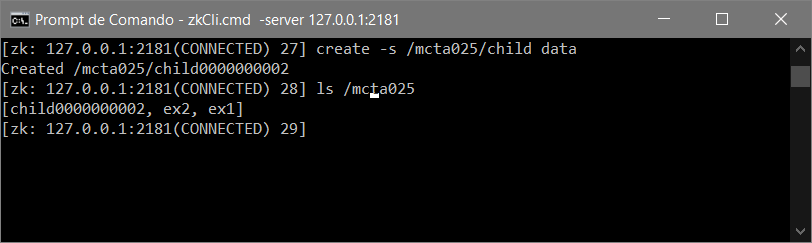
\includegraphics{pratica3/prints/roteiro 2.7.PNG}


\subsection*{3. Watches}
\addcontentsline{toc}{section}{3. Watches}

\subsubsection{3.1 - Todas as operaçõs de leitura no ZooKeeper tem a opção de se
configurar um watch. Abra um segundo cliente em paralelo, que
chamaremos de Cliente 2. O cliente inicial será chamado de Cliente 1.}
\addcontentsline{toc}{subsection}{3.1 Abra um segundo cliente em paralelo}

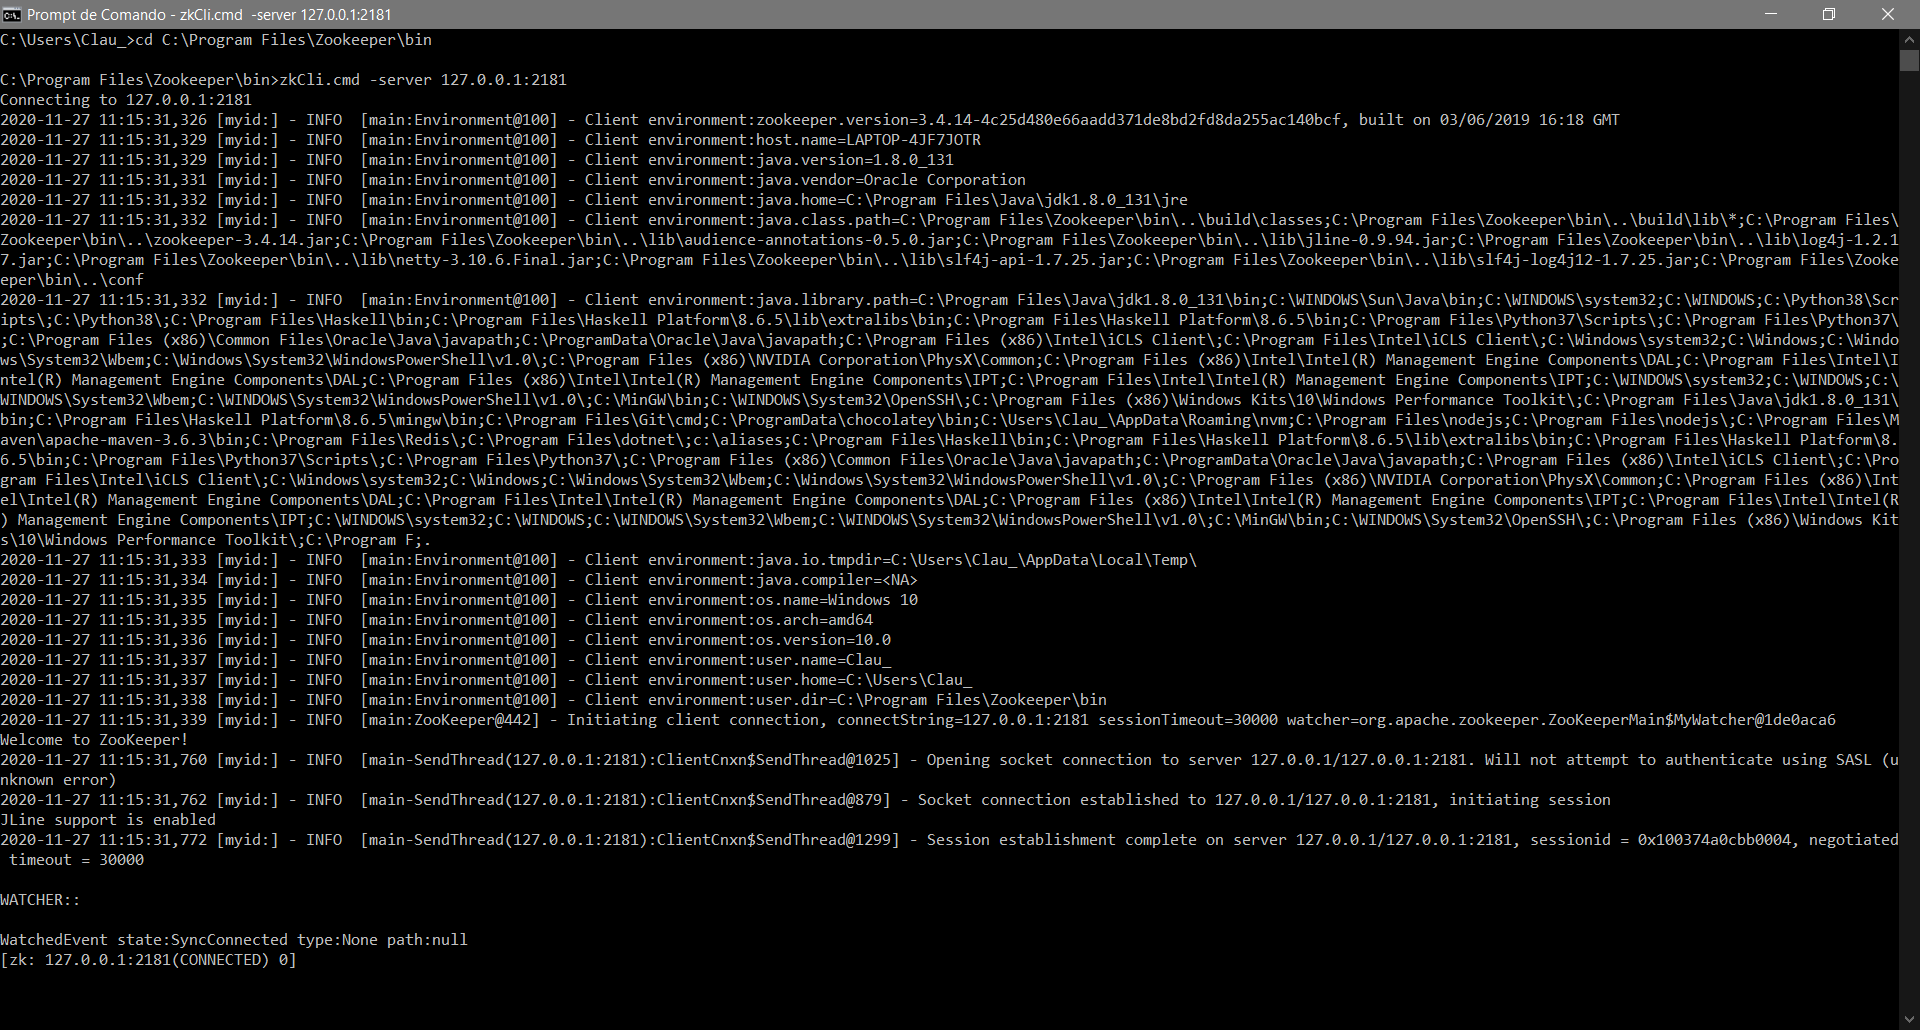
\includegraphics[width=20cm]{pratica3/prints/client2_started.PNG}

\subsubsection{3.2 - Crie um novo znode através do Cliente 1: create /mcta025/ex3
data.}
\addcontentsline{toc}{subsection}{3.2 Crie um novo znode através do Cliente 1}

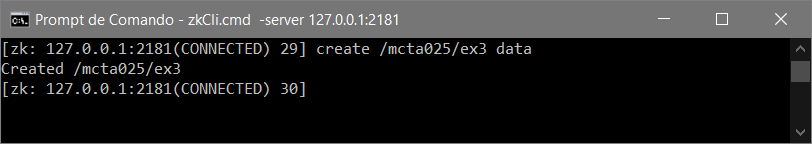
\includegraphics{pratica3/prints/roteiro 3.2.PNG}

\subsubsection{3.3 - Configure um watch de dados do nó que acabou de ser criado no
Cliente 1: get /mcta025/ex3 true}
\addcontentsline{toc}{subsection}{3.3 Configure um watch de dados do nó que acabou de ser criado no Cliente 1}

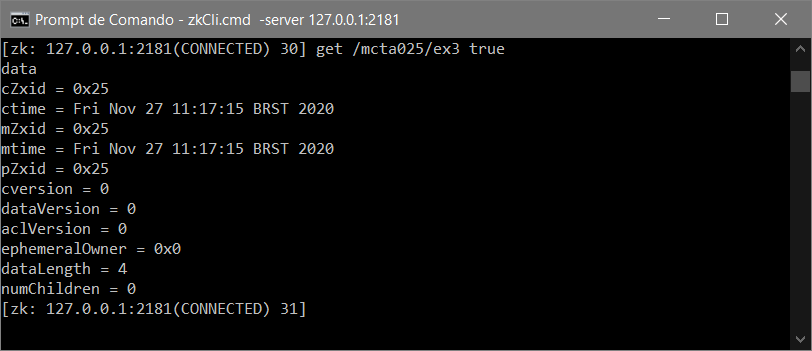
\includegraphics{pratica3/prints/roteiro 3.3.PNG}

\subsubsection{3.4 - No Cliente 2, modifique os dados do nó: set /mcta025/ex3
newData. O que acontece no Cliente 1?}
\addcontentsline{toc}{subsection}{3.4  Modifique os dados do nó no cliente 2}

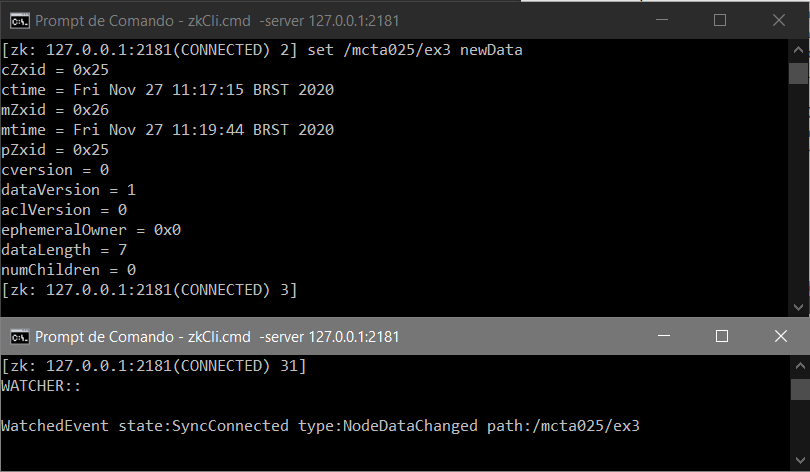
\includegraphics{pratica3/prints/roteiro 3.4.PNG}

\subsubsection{3.5 - Repita no Cliente 2 o comando anterior. O que aconteceu no Cliente 1? Justifique.}
\addcontentsline{toc}{subsection}{3.5 Repita no Cliente 2 o comando anterior}

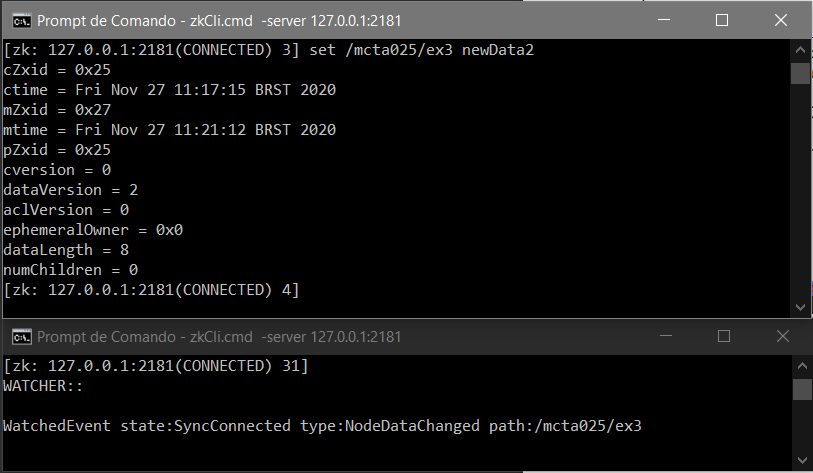
\includegraphics{pratica3/prints/roteiro 3.5.PNG}

\subsubsection{3.6 - É possível instalar watch de filhos de um nó. No Cliente 1: ls
/mcta025/ex3 true. Então, no Cliente 2, crie um novo filho dentro de /mcta025/ex3. O que aconteceu?}
\addcontentsline{toc}{subsection}{3.6 ?}

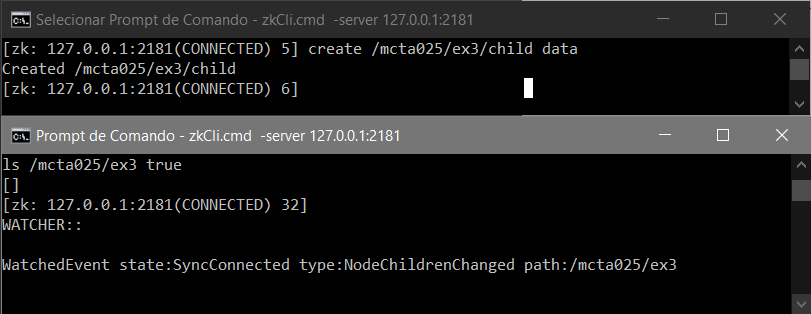
\includegraphics{pratica3/prints/roteiro 3.6.PNG}

\subsubsection{3.7 - Crie um watch de dados para /mcta025/ex3. No Cliente 2, crie um
filho em /mcta025/ex3. O que aconteceu? Justifique.}
\addcontentsline{toc}{subsection}{3.7 ?}

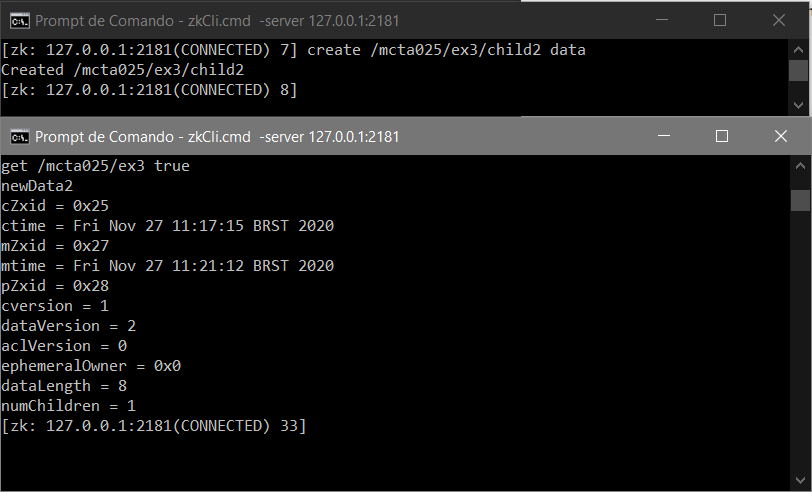
\includegraphics{pratica3/prints/roteiro 3.7.PNG}

\subsubsection{3.8 - Crie um watch de filhos para o nó /mcta025/ex3 e um watch de filhos para um filho dele usando o Cliente 1. No Cliente 2, crie um filho no
nó filho criado anteriormente. O que aconteceu? Agora crie um filho
em /mcta025/ex3. O que podemos concluir dessas operações?}
\addcontentsline{toc}{subsection}{3.8 ?}

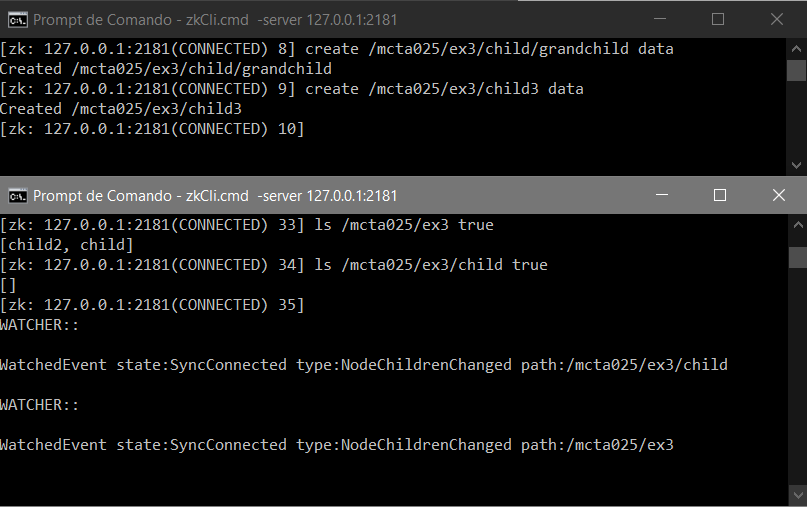
\includegraphics{pratica3/prints/roteiro 3.8.PNG}

\subsubsection{3.9 - Crie um watch de dados de um filho de /mcta025/ex3 e um watch de filhos para /mcta025/ex3 no Cliente 1. No Cliente 2, remova esse nó filho de /mcta025/ex3. O que aconteceu?}
\addcontentsline{toc}{subsection}{3.9 ?}

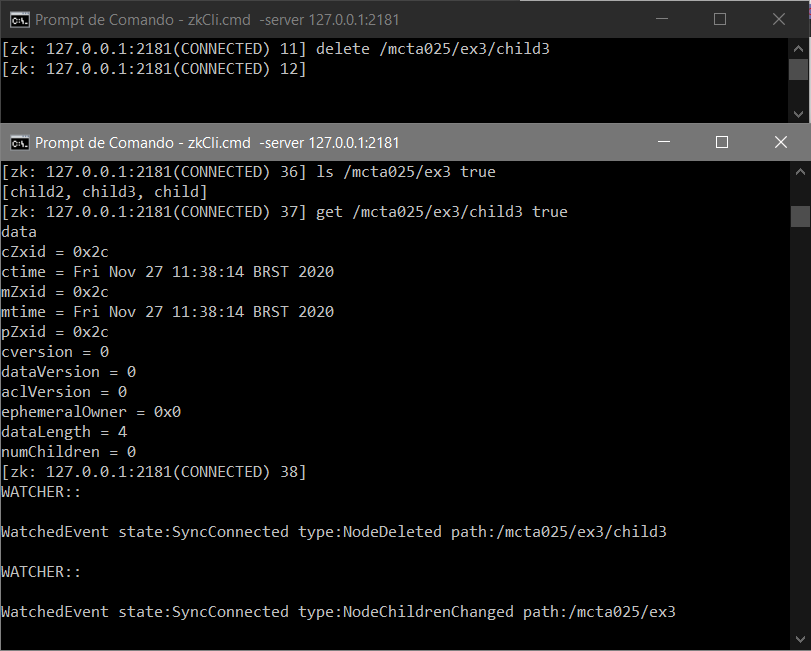
\includegraphics{pratica3/prints/roteiro 3.9.PNG}

\subsection*{4. ZooKeeper Java Example}
\addcontentsline{toc}{section}{4. ZooKeeper Java Example}


\subsubsection{4.1 - Execute o run.sh depois de acertar o valor da variável ZK para o diretório de instalação do ZooKeeper em seu computador.}
\addcontentsline{toc}{subsection}{4.1 ?}
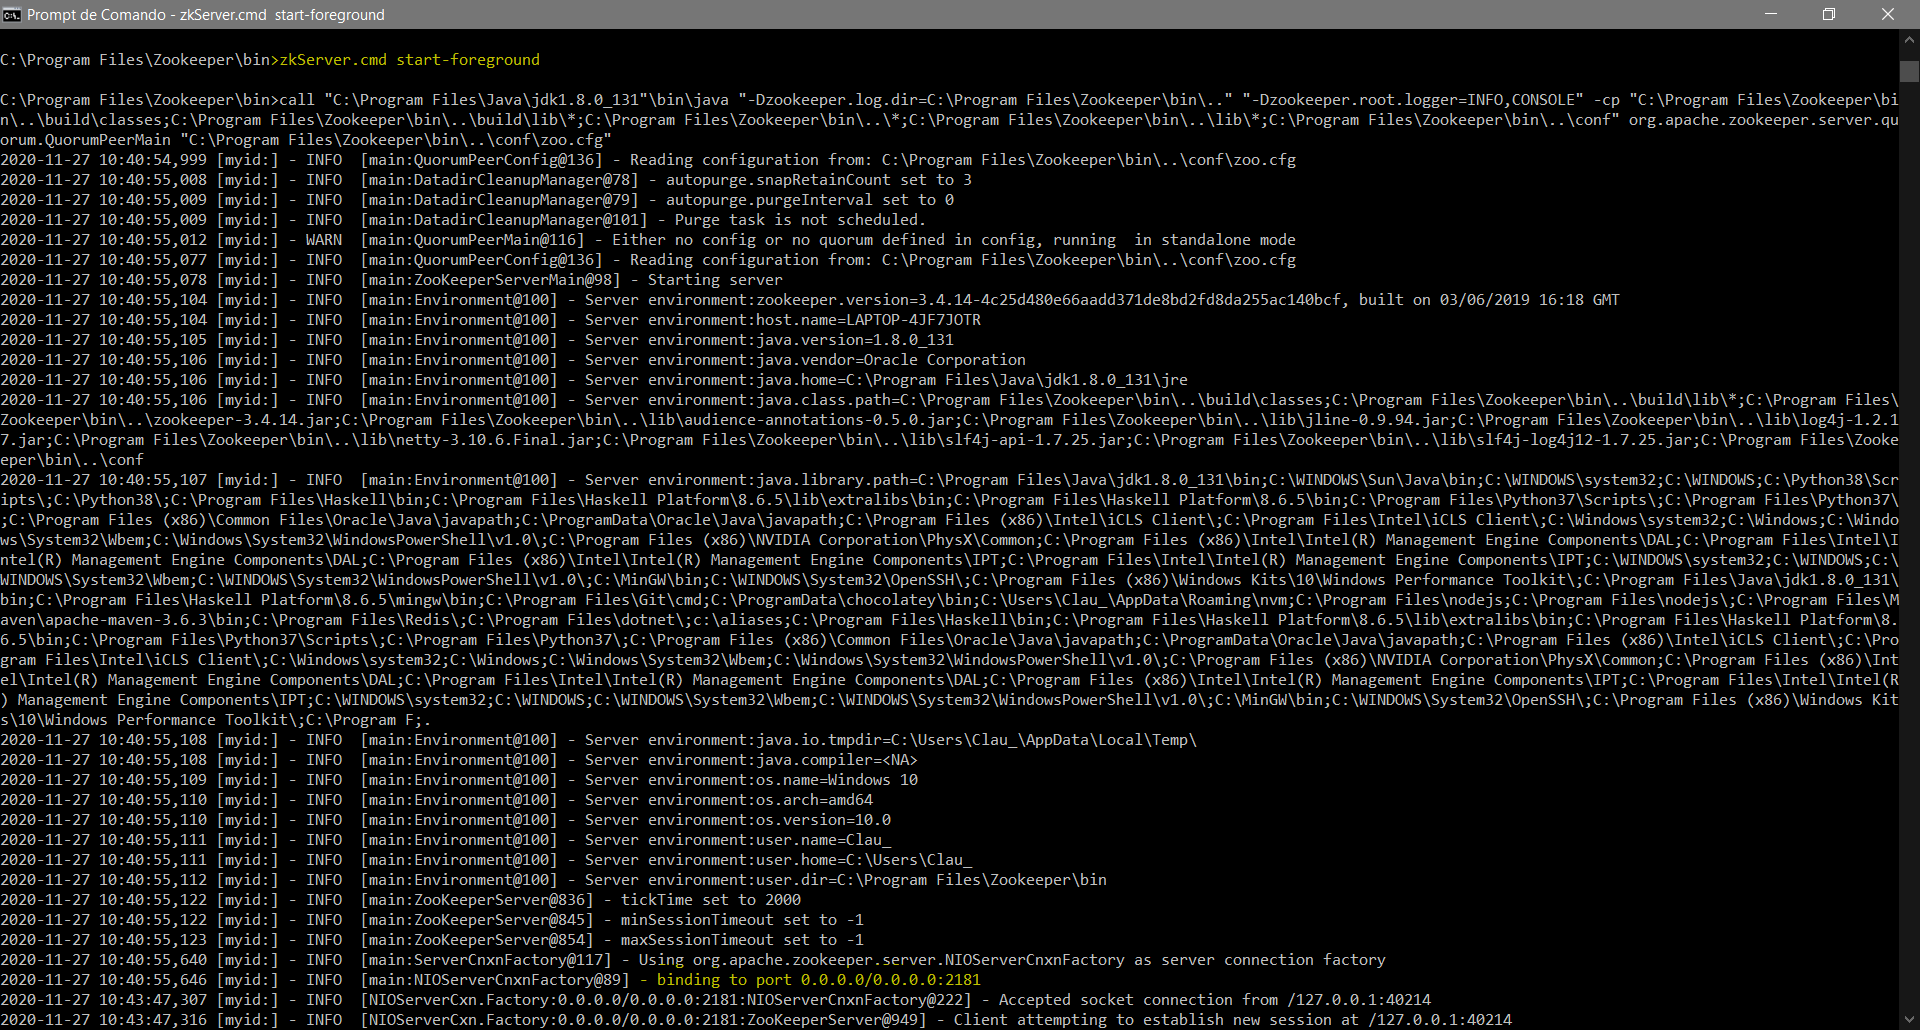
\includegraphics[width=20cm]{pratica3/prints/server_started.PNG}

\subsubsection{4.2 - Em uma CLI, crie um znode: create /mcta025/ex4 aData. O que
aconteceu?}
\addcontentsline{toc}{subsection}{4.2 Em uma CLI, crie um znode}

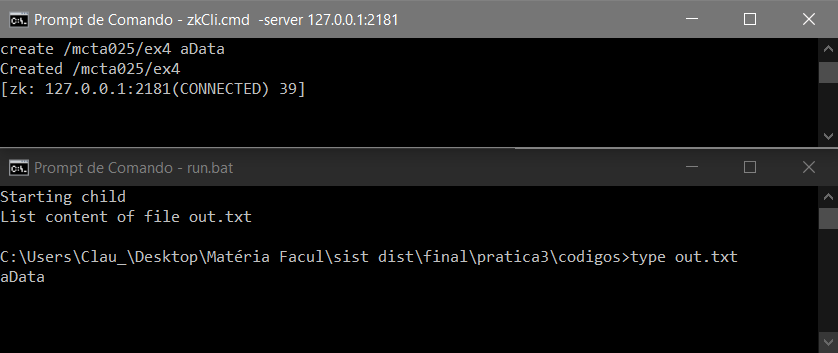
\includegraphics{pratica3/prints/roteiro 4.2.PNG}

\subsubsection{4.3 - Depois, mude o valor do nó: set /mcta025/ex4 newData. O que
aconteceu?}
\addcontentsline{toc}{subsection}{4.3 Depois, mude o valor do nó}
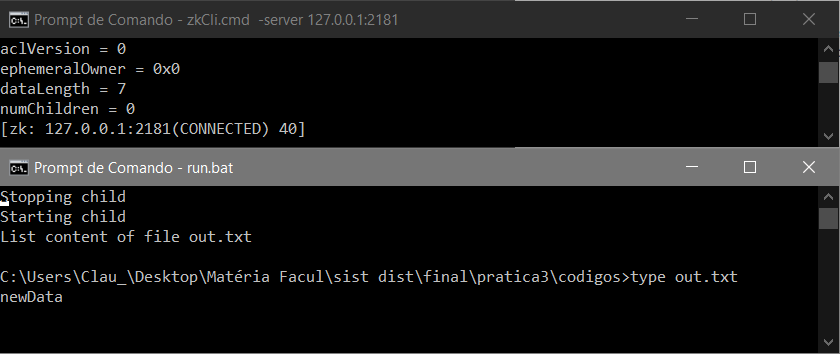
\includegraphics{pratica3/prints/roteiro 4.3.PNG}

\subsubsection{4.4 - Delete o nó: delete /mcta025/ex4. O que aconteceu?}
\addcontentsline{toc}{subsection}{4.4 Delete o nó}
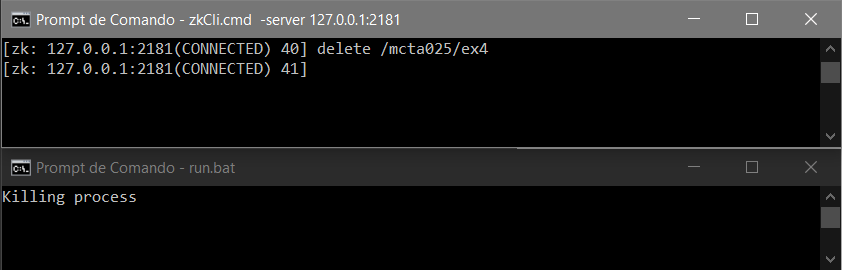
\includegraphics{pratica3/prints/roteiro 4.4.PNG}


\chapter*{Aula prática 4}
\addcontentsline{toc}{chapter}{Aula prática 4}
\subsection*{1. Barrier and Queue Tutorial.}
\addcontentsline{toc}{section}{1. Barrier and Queue Tutorial}

\subsubsection{1.1 - Modificar a variável ZK de acordo com a instalação do Zookeeper em run barrier.sh.}
\addcontentsline{toc}{subsection}{1.1 Modificar a variável ZK de acordo com a instalação do Zookeeper em run barrier.sh.}

\vspace{-0.5em}
\begin{minipage}{\textwidth}
  \hspace{-1em}
  \centering
  \lstinputlisting[language=sh]{pratica4/codigos/run_barrier.sh}
  \label{prog1}
  \hspace{1em}
\end{minipage}
\vspace{0.5em}

\subsubsection{1.2 - O que significa a variável SIZE em run barrier.sh?}
\addcontentsline{toc}{subsection}{1.2 O que significa a variável?}
A variável SIZE é o número mínimo de processos filhos para que o nó pai libere a computação de seu processo.

\subsubsection{1.3 - Executar run barrier.sh. O que aconteceu?}
\addcontentsline{toc}{subsection}{1.3 Executar run barrier.sh.}
Para entrar na barreira, um processo chama enter(). O processo cria um nó sob a raiz para representá-lo, usando seu nome de host para formar o nome do nó. Em seguida, aguarda até que processos suficientes tenham entrado na barreira. Um processo faz isso verificando o número de filhos que o nó raiz tem com "getChildren()" e esperando por notificações caso não haja o suficiente.
\newline
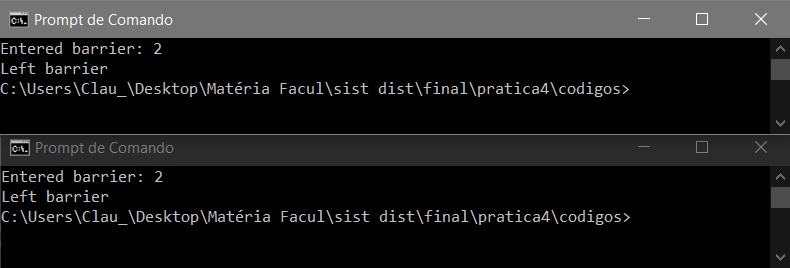
\includegraphics{pratica4/prints/roteiro 1.3.PNG}

\subsubsection{1.4 - Modificar a variável ZK de acordo com a instalação do Zookeeper em
run queue producer.sh.}
\addcontentsline{toc}{subsection}{1.4 Modificar a variável ZK de acordo com a instalação do Zookeeper em
run queue producer.sh.}

\vspace{-0.5em}
\begin{minipage}{\textwidth}
  \hspace{-1em}
  \centering
  \lstinputlisting[language=sh]{pratica4/codigos/run_queue_producer.sh}
  \label{prog1}
  \hspace{1em}
\end{minipage}
\vspace{0.5em}

\subsubsection{1.5 - Modificar a variável ZK de acordo com a instalação do Zookeeper em run queue consumer.sh.}
\addcontentsline{toc}{subsection}{1.5 Modificar a variável ZK de acordo com a instalação do Zookeeper em run queue consumer.sh.}

\vspace{-0.5em}
\begin{minipage}{\textwidth}
  \hspace{-1em}
  \centering
  \lstinputlisting[language=sh]{pratica4/codigos/run_queue_consumer.sh}
  \label{prog1}
  \hspace{1em}
\end{minipage}
\vspace{0.5em}

\subsubsection{1.6 - O que significa a variável SIZE em run queue producer.sh? E em
run queue consumer.sh?}
\addcontentsline{toc}{subsection}{1.6 O que significa a variável SIZE em run queue producer.sh? E em run queue consumer.sh?}
No run queue producer.sh, a variável SIZE corresponde ao número de elementos que serão colocados por ele na fila, enquanto que em run queue consumer, a variável SIZE corresponde ao número de elementos que serão consumidos da fila por ele.


\subsubsection{1.7 - Executar run queue consumer.sh e depois run queue producer.sh.
O que aconteceu? Alterne a execução dos scripts}
\addcontentsline{toc}{subsection}{1.7 Executar run queue consumer.sh e depois run queue producer.sh.}

O processo consumidor fica bloqueado se não houverem elementos para serem consumidos na fila (fica aguardando o produtor inserir esses elementos). Quando os elementos são adicionados ou já existem elementos na fila, o consumidor roda normalmente.
\newline

\begin{center}
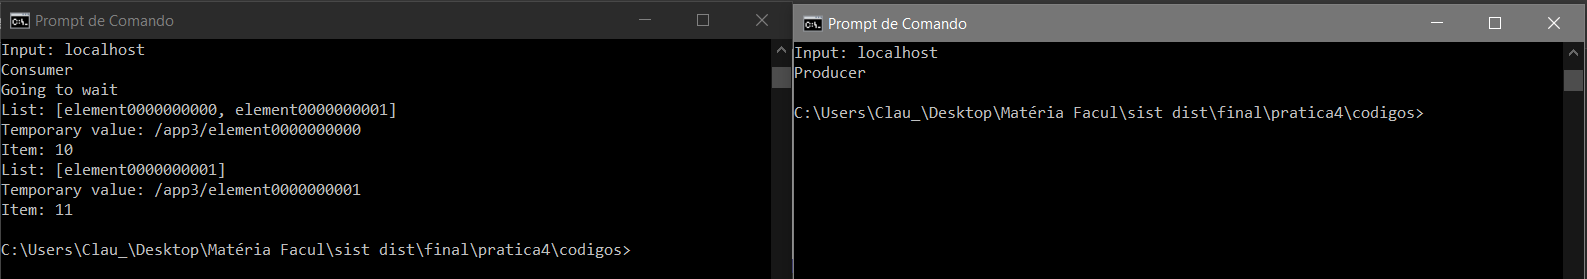
\includegraphics[width=20cm]{pratica4/prints/roteiro 1.7 c-p.PNG}
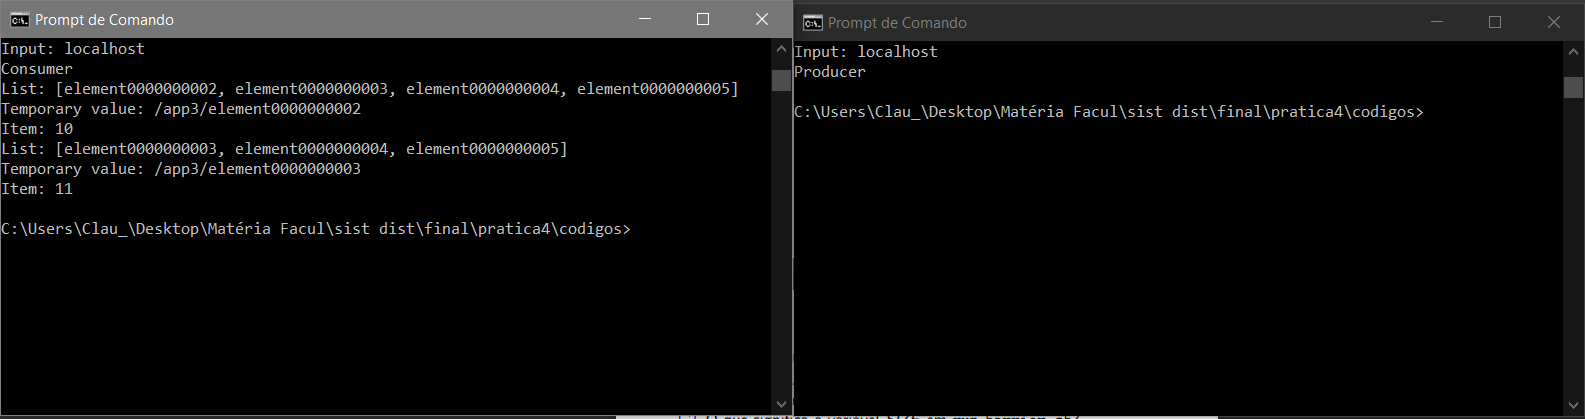
\includegraphics[width=20cm]{pratica4/prints/roteiro 1.7 p-p-c.PNG}
\end{center}

\subsection*{2. Tutorial de lock baseado no Barrier and Queue Tutorial}
\addcontentsline{toc}{section}{2. ?}

\subsubsection{2.1 - Modificar a variável ZK de acordo com a instalação do Zookeeper em run lock.sh.}
\addcontentsline{toc}{subsection}{2.1 Modificar a variável ZK de acordo com a instalação do Zookeeper em run lock.sh.}

\vspace{-0.5em}
\begin{minipage}{\textwidth}
  \hspace{-1em}
  \centering
  \lstinputlisting[language=sh]{pratica4/codigos/run_lock.sh}
  \label{prog1}
  \hspace{1em}
\end{minipage}
\vspace{0.5em}

\subsubsection{2.2 - O que significa a variável WAIT em run lock.sh?}
\addcontentsline{toc}{subsection}{2.2 O que significa a variável WAIT em run lock.sh?}

A variável WAIT corresponde ao tempo de espera para destravar o processo criado com o runlock.sh

\subsubsection{2.3 - Executar várias instâncias de run lock.sh. O que aconteceu?}
\addcontentsline{toc}{subsection}{2.3 Executar várias instâncias de run lock.sh}

LockService verifica se Entity já está bloqueado ou não usando a API de bloqueio de thread safe do ZooKeeper. Se a entidade já estiver bloqueada por qualquer outro thread de API (ou chamada), o LockService aguardará o período de tempo configurado. Para evitar a situação de conflito, o bloco sincronizado será colocado para cuidar do bloqueio de várias chaves de recursos.
\newline

\begin{center}
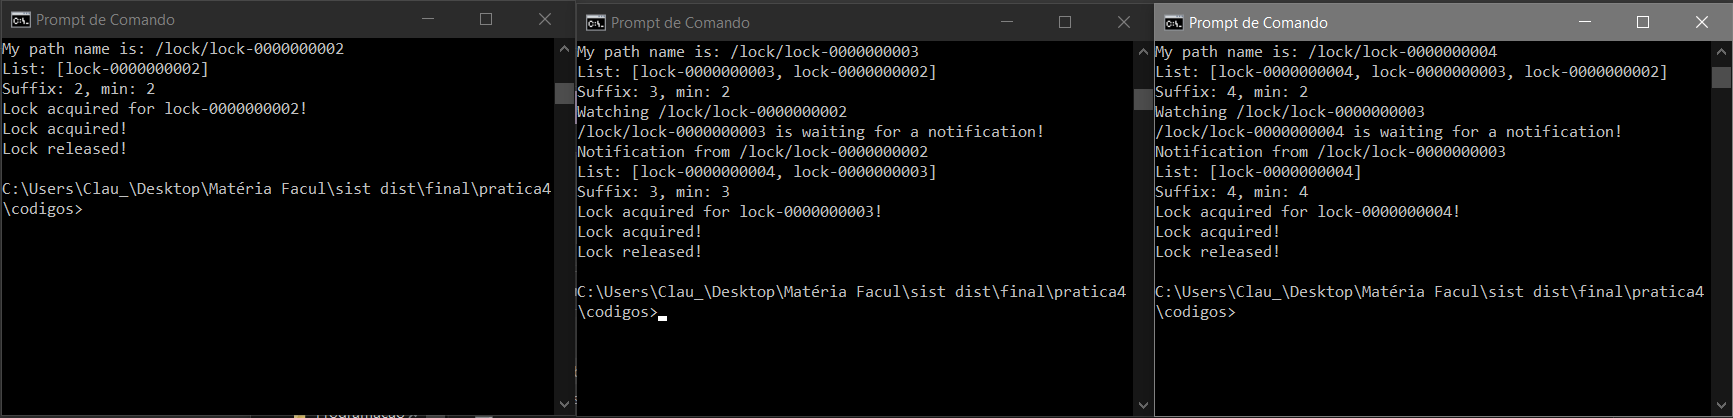
\includegraphics[width=20cm]{pratica4/prints/roteiro 2.3.PNG}
\end{center}

\subsubsection{2.4 - Executar várias instâncias de run lock.sh e, em seguida, matar
alguma instância intermediária. O que aconteceu?}
\addcontentsline{toc}{subsection}{2.4 Executar várias instâncias de run lock.sh e, em seguida, matar alguma instância intermediária}

Quando a lock intermediária é finalizada, o processo envia a notificação para o LockService, que atualiza a lista com as locks ativas e remove a intermediária da lista.
\newline
\begin{center}
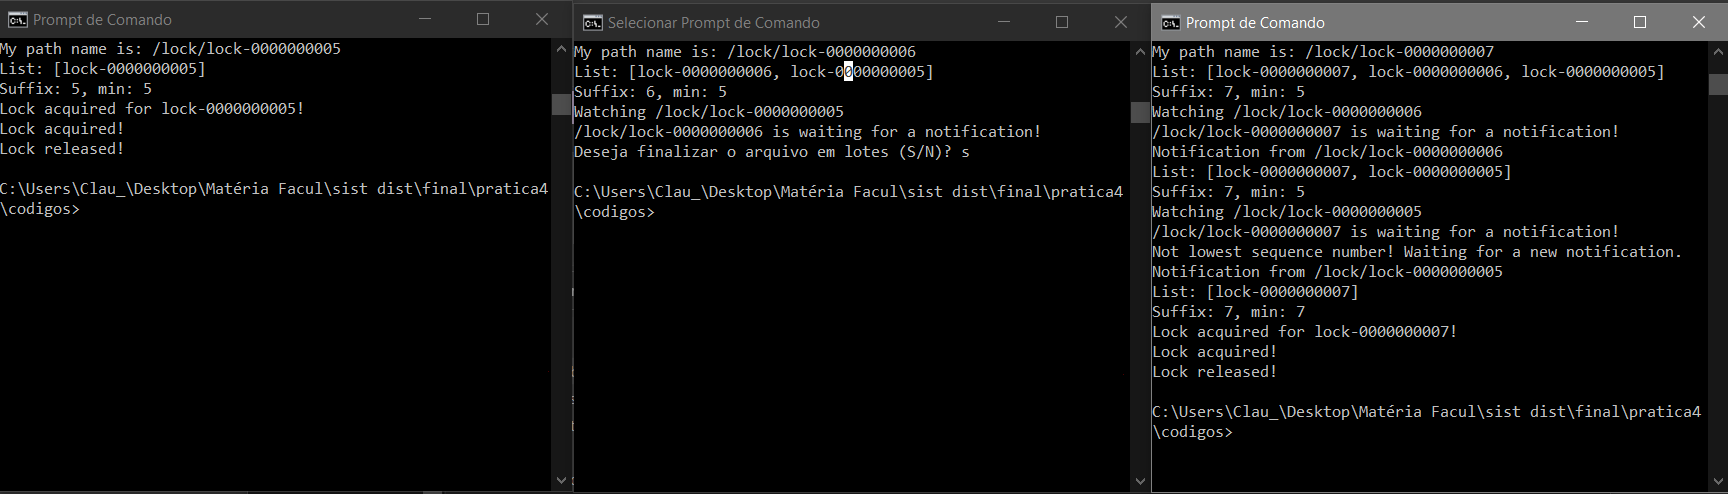
\includegraphics[width=20cm]{pratica4/prints/roteiro 2.4.PNG}
\end{center}

\chapter*{Aula prática 5}
\addcontentsline{toc}{chapter}{Aula prática 5}
\subsection*{1. Implementando eleição de coordenador}
\addcontentsline{toc}{section}{1. Implementando eleição de coordenador}

\subsubsection{1.1 -Modificar a variável ZK de acordo com a instalação do Zookeeper em
run leader.sh. Assegurar que exista um servidor do Zookeeperfuncionando localmente.}
\addcontentsline{toc}{subsection}{1.1 Modificar a variável ZK de acordo com a instalação do Zookeeper em run leader.sh.}

\vspace{-0.5em}
\begin{minipage}{\textwidth}
  \hspace{-1em}
  \centering
  \lstinputlisting[language=sh]{pratica5/codigos/run_leader.sh}
  \label{prog1}
  \hspace{1em}
\end{minipage}
\vspace{0.5em}

\subsubsection{1.2 - Executar várias instâncias de run leader.sh. O que aconteceu?}
\addcontentsline{toc}{subsection}{1.2 Executar várias instâncias de run leader.sh.}

Conforme o processo líder mais antigo morre, o próximo líder é o processo que está olhando para o znode mais antigo que os demais restantes. \newline

\begin{center}
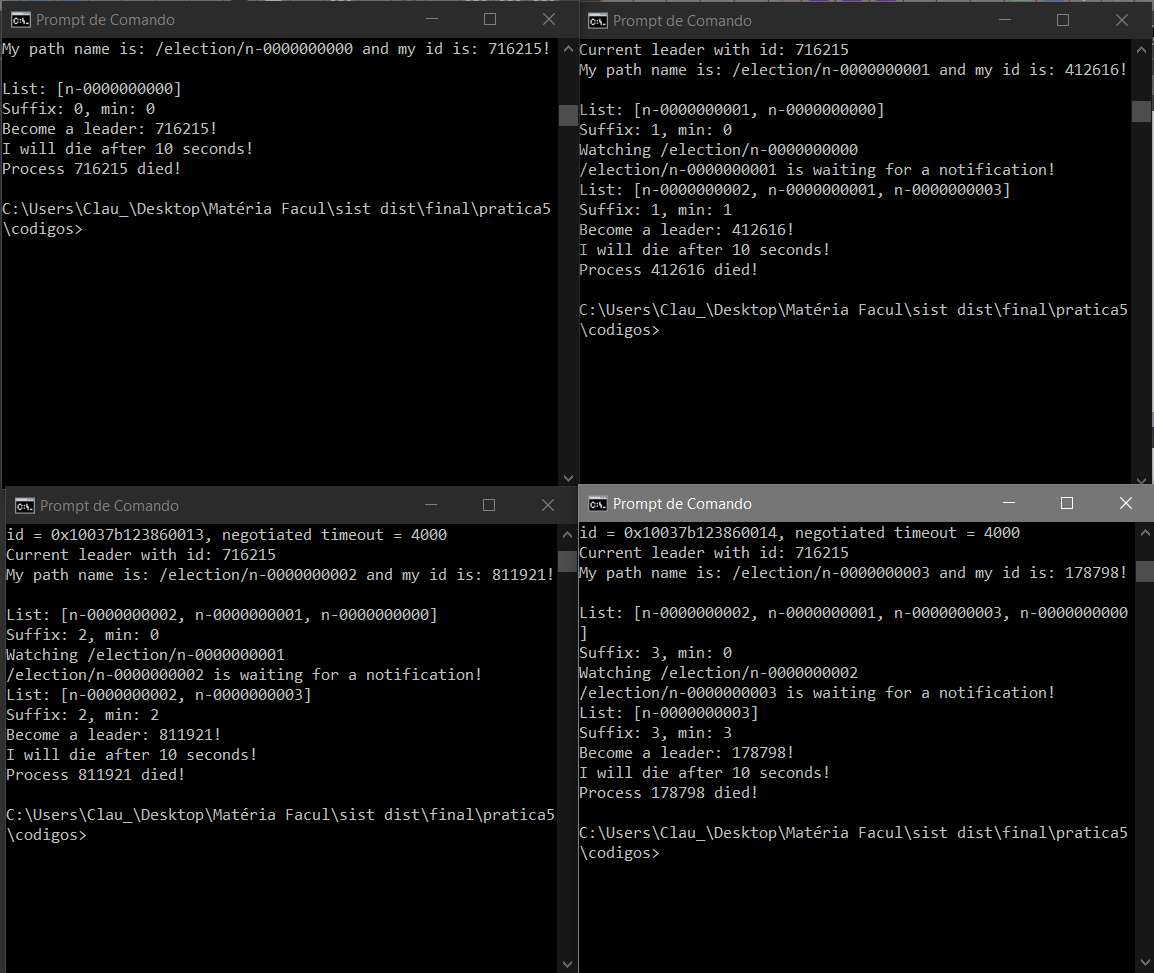
\includegraphics[width=20cm]{pratica5/prints/roteiro 1.2.PNG}
\end{center}

\subsubsection{1.3 - Executar várias instâncias de run leader.sh e, em seguida, matar
alguma instância intermediária. O que aconteceu?}
\addcontentsline{toc}{subsection}{2.4 Executar várias instâncias de run leader.sh. e, em seguida, matar alguma instância intermediária}

A fila é refeita após o processo intermediário ser finalizado. A cadeia de execução continua sendo executada normalmente, até o último processo que foi criado. \newline

\begin{center}
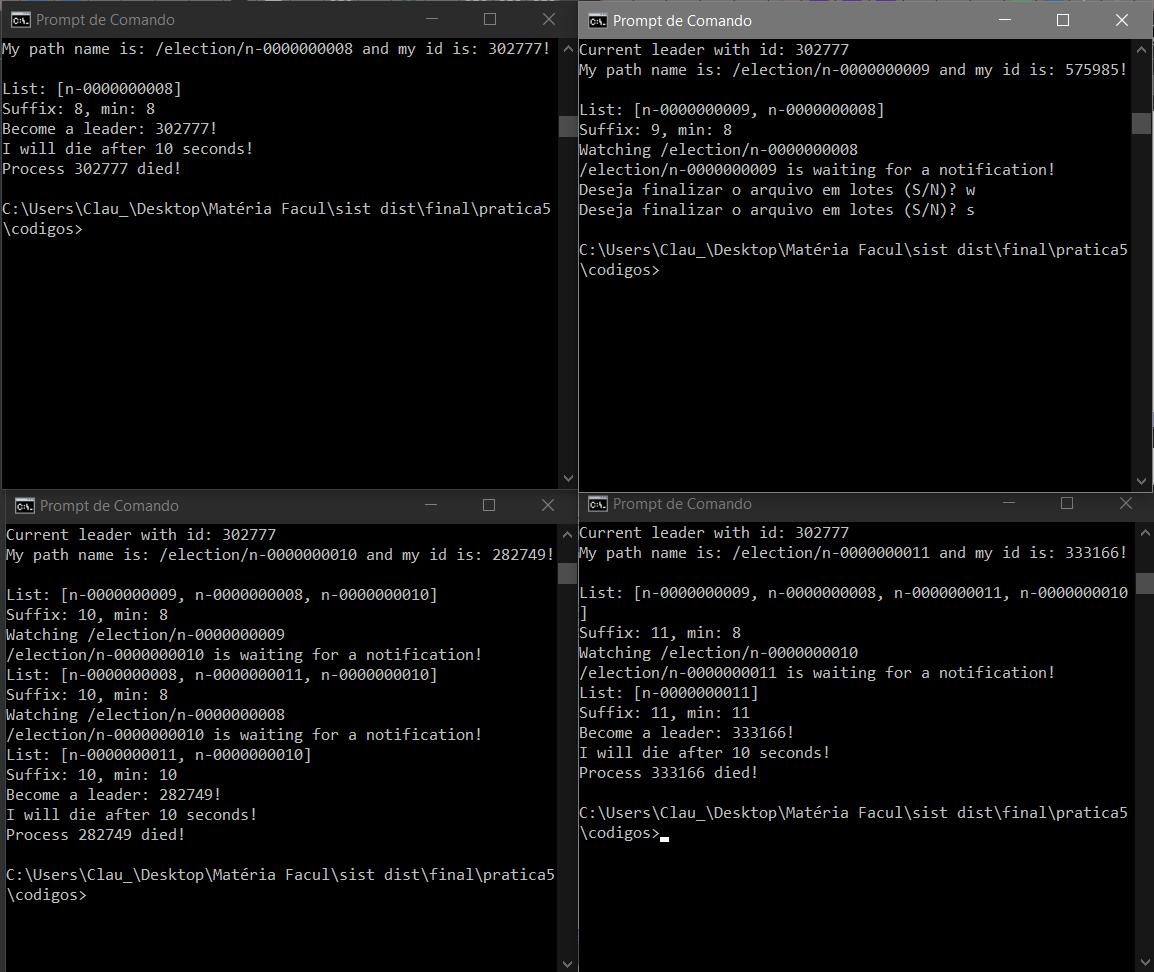
\includegraphics[width=20cm]{pratica5/prints/roteiro 1.3.PNG}
\end{center}

\subsection*{2. Criando um cluster para o Zookeeper – ensemble.}
\addcontentsline{toc}{section}{2. Criando um cluster para o Zookeeper}



\chapter*{Projeto Final}
\addcontentsline{toc}{chapter}{Projeto Final}
\setlength{\parindent}{4em}
\setlength{\parskip}{1em}

O nosso projeto consiste em um serviço de bate papo online, que possui, além do chat online, a opção de criar salas de reunião. A implementação do sistema foi feita em Java, aproveitando os códigos do Zookeeper que vimos em aula.\par
Para ligar o chat, faz-se necessário configurar o Zookeeper na máquina (como feito nas aulas práticas) e executar o arquivo ClientCLI.java. Esse arquivo é responsável por organizar o ambiente de usuário de maneira intuitiva, afim de facilitar a interação entre o usuário e o sistema. Dentro da CLI, o usuário tem as seguintes opções de comando:
\begin{itemize}
	\item entrar
	\par Entra numa sala de reunião.
	\item criar
	\par Cria uma sala de reunião nova.
	\item sair
	\par Sai da sala de reunião atual.
	\item ajuda
	\par Lista os comandos possíveis de serem executados e como usá-los.
	\item enviar
	\par Envia mensagem num chat individual ou reunião.
	\item receber
	\par Primeiro faz a busca de mensagens antigas (enviadas antes do usuário fazer login) e depois fica esperando a notificação de mensagens novas.
	\item parar
	\par Comando para parar de esperar a notificação de mensagens novas.
	\item transmitir
	\par Inicia a transmissão de conteúdo dentro da sala de reunião.
	\item chat
	\par Especifica o tipo de mensangem que o usuário quer enviar.
	\item reuniao
	\par Especifica o tipo de sala que o usuário quer se conectar.
\end{itemize}
\par
Aqui está a representação de uma sala chat funcionando. Fazemos o login com 4 usuários diferentes e fazemos 3 deles enviar uma mensagem para o mesmo usuário ("mario"). Ele aguarda o recebimento das mensagens e é notificado:
\begin{center}
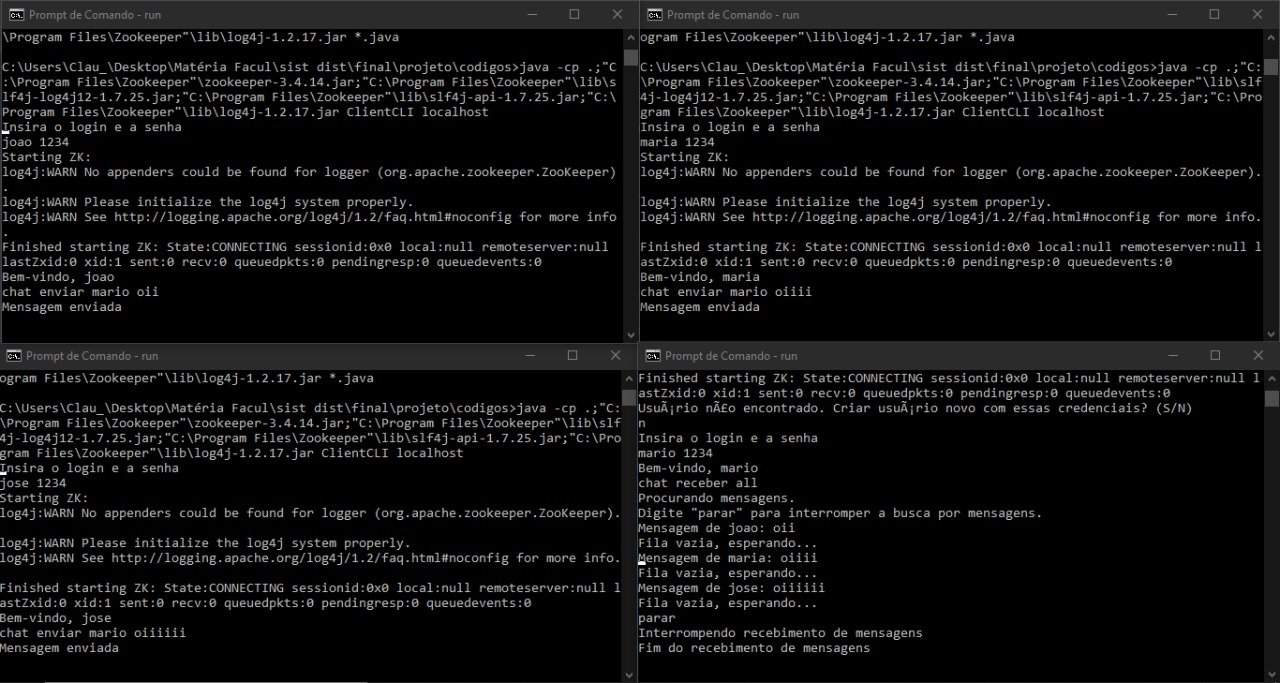
\includegraphics[width=20cm]{projeto/prints/exemplo-chat1.jpeg}
\end{center}

\par Exemplo de reunião. O primeiro usuário cria a sala de reunião e ele é o líder da sala. Os demais conectam na sala e o líder inicia a sua apresentação. Quando o líder sai da sala, um novo líder é eleito e esse novo líder pode iniciar sua apresentação.

\begin{center}
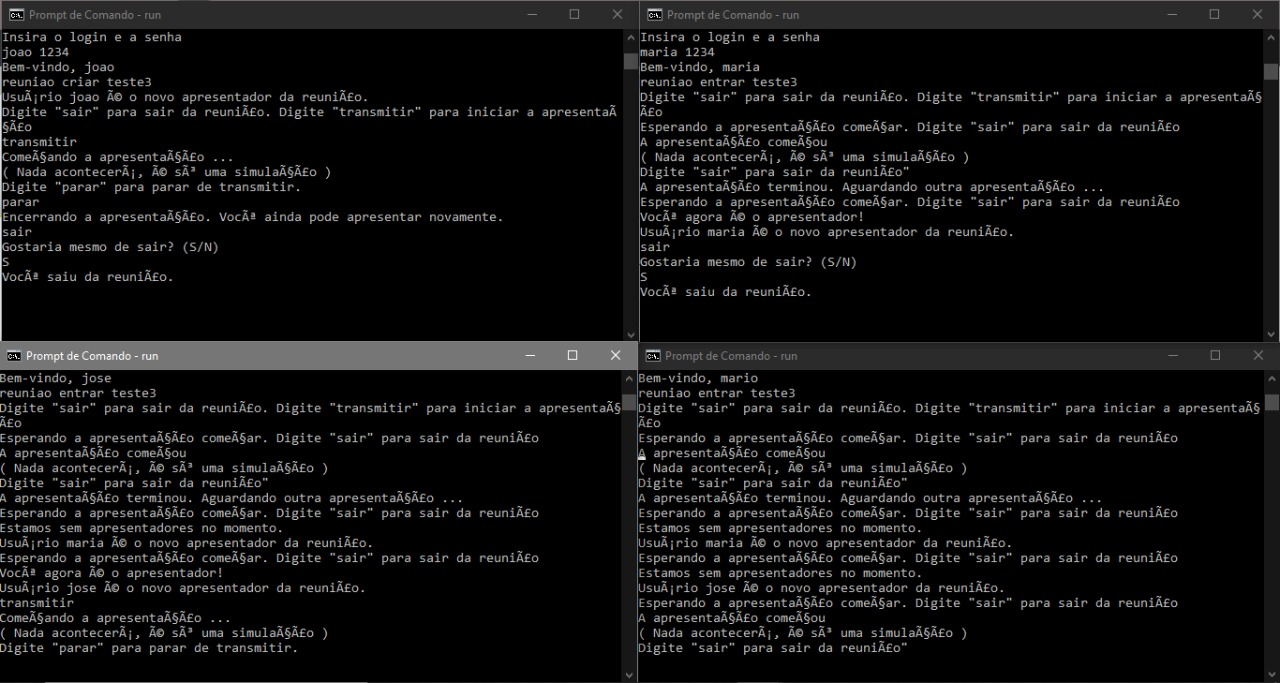
\includegraphics[width=20cm]{projeto/prints/exemplo-reuniao1.jpeg}
\end{center}


\end{document}